\documentclass{memoir}

\usepackage{amsthm,amssymb,amsmath}
\usepackage{makeidx}
\usepackage{xifthen}
\usepackage[inline]{enumitem}
\usepackage{tikz}
  \usetikzlibrary{patterns}
  \usetikzlibrary{cd}
  \usetikzlibrary{calc}
  \usetikzlibrary{arrows}
\usepackage[framemethod=tikz,usetwoside]{mdframed}
\usepackage{hyperref}
  \hypersetup{linktocpage,colorlinks,linkcolor=blue}
\usepackage[figurewithin=section]{caption}
\usepackage{collect}
\usepackage{wasysym}
\usepackage{mathtools}

% #Counters
%

%-----------%
% #Counters %
%-----------%

% Number chapters as I, II, III, etc.
\renewcommand{\thechapter}{\Roman{chapter}}

% Number sections sequentially (not within chapters)
\counterwithout{section}{chapter}

% Number figures and tables within sections
\makeatletter                        %&%
  \renewcommand\@memmain@floats{     %&%
    \counterwithout{figure}{chapter} %&%
    \counterwithin{figure}{section}  %&%
    \counterwithout{table}{chapter}  %&%
    \counterwithin{table}{section}   %&%
  }                                  %&%
\makeatother                         %&%




%%%


% Keep chapter numbers and titles from overlapping in TOC
\renewcommand{\chapternumberlinebox}[2]{\makebox[1cm][l]{#2}}

% Roman-enumerated lists for propositions and proofs
\newenvironment{proplist}[0] %&%
  {\begin{enumerate}[(i)]}   %&%
  {\end{enumerate}}          %&%

\newenvironment{proplist*}[0]                        %&%
  {\begin{enumerate}[(i)] \setlength{\itemsep}{0pt}} %&%
  {\end{enumerate}}                                  %&%

\newenvironment{inlineproplist}[0] %&%
  {\begin{inparaenum}[(i)]}        %&%
  {\end{inparaenum}}               %&%

% Subreferences
\newcommand{\sref}[2]{\ref{#1}(\ref{#1:#2})}
\newcommand{\paref}[1]{(\ref{#1})}
\newcommand{\eref}[1]{\hyperref[#1]{Exercise \ref*{#1}}}
\newcommand{\propref}[1]{\hyperref[#1]{Proposition \ref*{#1}}}


% Page style
\makepagestyle{standard} %&%

\makeatletter                                                  %&%
\makeevenfoot{standard}{}{}{}                                  %&%
\makeoddfoot{standard}{}{}{}                                   %&%
\makeevenhead{standard}{\bfseries\thepage}{}{\rightmark}       %&%
\makeoddhead{standard}{\leftmark}{}{\bfseries\thepage}         %&%
\makeheadrule{standard}{\textwidth}{\normalrulethickness}      %&%
\makefootrule{standard}{\textwidth}{\normalrulethickness}{0ex} %&%
\makeatother                                                   %&%

\renewcommand*{\sectionmark}[1]{                      %&%
  \markboth{\S\thesection: {#1}}{\S\thesection: {#1}} %&%
}                                                     %&%

\nouppercaseheads    %&%
\pagestyle{standard} %&%
\chapterstyle{dash}  %&%

% Theorem styles
\theoremstyle{definition}                 %&%
\newtheorem{dfn}{Def'n}[section]          %&%
\newtheorem{thm}[dfn]{Theorem}            %&%
\newtheorem{cor}[dfn]{Cor.}               %&%
\newtheorem{prop}[dfn]{Prop'n}            %&%
\newtheorem{lem}[dfn]{Lemma}              %&%
\newtheorem{construct}[dfn]{Construction} %&%
\newtheorem{axiom}[dfn]{Axiom}            %&%

% Exercises
\newcommand{\Exercises}{\par\bigskip\noindent\hfill{\textasteriskcentered\quad\textasteriskcentered\quad\textsc{\large Exercises}\quad\textasteriskcentered\quad\textasteriskcentered}\hfill\null\par\bigskip}

\newcounter{dummycounter}         %&%
\newcounter{exercise}[section]    %&%
\counterwithin{exercise}{section} %&%

\marginparmargin{left} %&%

\newenvironment{exercise}[1][\unskip]{                     %&%
  \refstepcounter{exercise}                                %&%
  \par\noindent\marginpar{\hfill\theexercise .}\textbf{#1} %&%
}{                                                         %&%
  \medskip                                                 %&%
}                                                          %&%



% Examples
\newenvironment{examples}{                      %&%
  \par\bigskip\noindent\textbf{\large Examples} %&%
  \begin{enumerate}                             %&%
}{                                              %&%
  \end{enumerate}                               %&%
}                                               %&%


\mdfdefinestyle{mystyle}{ %&%
  hidealllines=true,      %&%
  leftline=true,          %&%
  innerleftmargin=10pt,   %&%
  innerrightmargin=10pt,  %&%
  innertopmargin=0pt,     %&%
}                         %&%

\surroundwithmdframed[style=mystyle]{dfn}   %&%
\surroundwithmdframed[style=mystyle]{prop}  %&%
\surroundwithmdframed[style=mystyle]{cor}   %&%
\surroundwithmdframed[style=mystyle]{axiom} %&%

\def\chapterautorefname{Chapter} %&%
\def\sectionautorefname{Section} %&%
\def\figureautorefname{Figure}   %&%


% For nebulous "problem" statements
\newenvironment{titlebox}[1]                       %&%
  {\mdfsetup{                                      %&%
    frametitle={\colorbox{white}{\space#1\space}}, %&%
    innertopmargin=7pt,                            %&%
    innerbottommargin=10pt,                        %&%
    frametitleaboveskip=-\ht\strutbox,             %&%
    frametitlealignment=\center                    %&%
    }                                              %&%
  \begin{mdframed}                                 %&%
  }                                                %&%
  {\end{mdframed}                                  %&%
}                                                  %&%


%---------%
% Numbers %
%---------%

\newcommand{\ZZ}{\ensuremath{\mathbb{Z}}} %&%
\newcommand{\NN}{\ensuremath{\mathbb{N}}} %&%
\newcommand{\QQ}{\ensuremath{\mathbb{Q}}} %&%
\newcommand{\RR}{\ensuremath{\mathbb{R}}} %&%
\newcommand{\CC}{\ensuremath{\mathbb{C}}} %&%

\newcommand{\ZZINT}[2]{\ensuremath{[\![#1,#2]\!]}} %&%



%-----------------------%
% Maps and sets of maps %
%-----------------------%

\newcommand{\ID}[1][]{\ensuremath{ %&%
  \ifthenelse{\isempty{#1}}        %&%
    {\mathsf{id}}                  %&%
    {\mathsf{id}_{#1}}             %&%
}}                                 %&%

\newcommand{\END}[1]{\ensuremath{ %&%
  \mathsf{End}\left(#1\right)     %&%
}}                                %&%

\newcommand{\ENDU}[1]{\ensuremath{ %&%
  \mathsf{End}_1\left(#1\right)    %&%
}}                                 %&%



%--------------%
% Ring subsets %
%--------------%

\newcommand{\CENTER}[1]{\ensuremath{ %&%
  Z\left(#1\right)                   %&%
}}                                   %&%

\newcommand{\NILRADICAL}[1]{\ensuremath{ %&%
  N\left(#1\right)                       %&%
}}                                       %&%

\newcommand{\UNITS}[1]{\ensuremath{ %&%
  \mathcal{U}\left(#1\right)        %&%
}}                                  %&%

\newcommand{\KER}[1]{\ensuremath{ %&%
  \mathsf{ker}(#1)                %&%
}}                                %&%

\newcommand{\IM}[1]{\ensuremath{ %&%
  \mathsf{im}(#1)                %&%
}}                               %&%



%--------------------------%
% Families of ring subsets %
%--------------------------%

\newcommand{\ASSOCLAT}[1]{\ensuremath{ %&%
  \mathcal{A}\left(#1\right)           %&%
}}                                     %&%

\newcommand{\IDEALS}[2][]{\ensuremath{ %&%
  \ifthenelse{\isempty{#1}}            %&%
    {\mathcal{Q}\left(#2\right)}       %&%
    {\mathcal{Q}_{#1}\left(#2\right)}  %&%
}}                                     %&%



%----------%
% Geometry %
%----------%

\newcommand{\COLLINEAR}[3]{\ensuremath{\langle #1, #2, #3 \rangle}}%&%
\newcommand{\LINE}[2]{\ensuremath{\overleftrightarrow{#1#2}}}%&%
\newcommand{\BETWEEN}[3]{\ensuremath{[ #1 #2 #3 ]}}%&%
\newcommand{\SEGMENT}[2]{\ensuremath{\overline{#1#2}}}%&%
\newcommand{\RAY}[2]{\ensuremath{\overrightarrow{#1#2}}}%&%
\newcommand{\TRIANGLE}[3]{\ensuremath{\bigtriangleup{#1#2#3}}}%&%
\newcommand{\ANGLE}[3]{\ensuremath{\angle{#1#2#3}}}%&%
\newcommand{\INTANGLE}[3]{\ensuremath{\mathsf{int}\angle{#1#2#3}}}%&%
\newcommand{\SEGCONG}[4]{\ensuremath{(#1,#2) \cong_s (#3,#4)}}%&%
\newcommand{\ANGCONG}[6]{\ensuremath{(#1,#2,#3) \cong_a (#4,#5,#6)}}%&%
\renewcommand{\CIRCLE}[2]{\ensuremath{\ocircle{#1#2}}}%&%
\newcommand{\INTCIRCLE}[2]{\ensuremath{\mathsf{int}\CIRCLE{#1}{#2}}}
\newcommand{\EXTCIRCLE}[2]{\ensuremath{\mathsf{ext}\CIRCLE{#1}{#2}}}

\newcommand{\HALFPLANEA}[1]{\mathcal{H}_{1,\ell}}
\newcommand{\HALFPLANEB}[1]{\mathcal{H}_{2,\ell}}

\newcommand{\SEPARATE}[4]{\ensuremath{(#1,#2 \mid #3,#4)}}

\newcommand{\HYPHP}{\ensuremath{\mathbb{H}}}
\newcommand{\HHPIDEALPOINT}[2]{\ensuremath{H_{#1,#2}}}

\newcommand{\POINCAREDISC}{\ensuremath{\mathbb{P}}}
\newcommand{\PDDET}[2]{D_{#1,#2}}
\newcommand{\PDIDEALPOINT}[2]{P_{#1,#2}}

\newcommand{\KLEINDISC}{\ensuremath{\mathbb{K}}}
\newcommand{\KDIDEALPOINT}[2]{\ensuremath{K_{#1,#2}}}

\newcommand{\EUCLIDEANDISC}{\ensuremath{\mathbb{E}}}

\newcommand{\ANTIPODALSPHERE}{\ensuremath{\mathbb{A}}}

\newcommand{\MIN}{\ensuremath{\mathsf{min}}}
\newcommand{\MAX}{\ensuremath{\mathsf{max}}}



\newcommand{\SYM}[1]{\ensuremath{\mathsf{Sym}(#1)}}



\newcommand{\TOT}[1]{\ensuremath{\mathsf{tot}\left(#1\right)}}%&%

\newcommand{\POW}[1]{\ensuremath{\mathcal{P}\left(#1\right)}}%&%
\newcommand{\POWP}[1]{\ensuremath{\mathcal{P}_{\!\neq\!}\left(#1\right)}}%&%
\newcommand{\POWF}[1]{\ensuremath{\mathcal{P}_F\left(#1\right)}}%&%

\newcommand{\ZZQUAD}[1]{\ensuremath{\mathcal{O}(\sqrt{#1})}}%&%
\newcommand{\ZZFRAC}[1]{\ensuremath{{#1}^{-1}\ZZ}}%&%

\newcommand{\ION}[1]{\ensuremath{\mathsf{nilp}\left(#1\right)}}%&%

\newcommand{\REXTEND}[3]{\ensuremath{#1 \rtimes_{#2} #3}}%&%
\newcommand{\ADJUNIT}[1]{\ensuremath{{#1}^{(1)}}}%&%
\newcommand{\HAM}[1]{\ensuremath{\mathbb{H}(#1)}}%&%

\newcommand{\ADDORD}[1]{\ensuremath{\mathsf{ord}\left(#1\right)}}%&%
\newcommand{\CHAR}[1]{\ensuremath{\mathsf{char}(#1)}}%&%

\newcommand{\MAT}[2]{\ensuremath{\mathsf{Mat}_{#1}(#2)}}%&%
\newcommand{\UTMAT}[2]{\ensuremath{\mathsf{UT}_{#1}(#2)}}%&%
\newcommand{\LTMAT}[2]{\ensuremath{\mathsf{LT}_{#1}(#2)}}%&%
\newcommand{\DIAGMAT}[2]{\ensuremath{\mathsf{Diag}_{#1}(#2)}}%&%
\newcommand{\DET}{\ensuremath{\mathsf{det}}}%&%

\newcommand{\GCD}[2]{\ensuremath{\mathsf{gcd}(#1, #2)}}%&%
\newcommand{\LCM}[2]{\ensuremath{\mathsf{lcm}(#1, #2)}}%&%
\newcommand{\GCDS}[1]{\ensuremath{\mathsf{gcd}\left(#1\right)}}%&%

\newcommand{\CONTENT}[1]{\ensuremath{\mathsf{content}(#1)}}%&%

\newcommand{\ASSOC}{\ensuremath{\approx}}%&%
\newcommand{\COPRIME}{\ensuremath{\perp}}%&%

\newcommand{\DIVORD}[2]{\ensuremath{\mathsf{div}_{#1}\left(#2\right)}}%&%

\newcommand{\LOCALIZE}[2]{\ensuremath{{#2}^{-1}{#1}}}%&%

\newcommand{\POLYEVAL}[1]{\ensuremath{\varepsilon_{#1}}}%&%
\newcommand{\DERIV}[1][]{\ensuremath{\ifthenelse{\isempty{#1}}{\mathsf{D}}{\mathsf{D}_{#1}}}}%&%

\newcommand{\TILDE}[1]{\ensuremath{\widetilde{#1}}}%&%

\newcommand{\LIM}[2][]{\ensuremath{\ifthenelse{\isempty{#1}}{\lim}{\lim_{#1}}\left(#2\right)}}%&%

\newcommand{\VALCOMP}[2]{\ensuremath{\overline{#1}_{#2}}}%&%


\makeindex

\begin{document}

\title{Elementary Geometrese}
\author{nathan bloomfield}


\frontmatter
  \maketitle

  \tableofcontents


\mainmatter
  \section{Models and Theories}
    One of the goals of this class is to explore the classical theory of geometry as laid out in the famous \emph{Elements of Geometry} by the Greek mathematician Euclid.
Before we begin, though, a few words about the distinction between a \emph{theory} and a \emph{model} are in order.

\begin{itemize}
\item A \textbf{theory} consists of one or more \emph{undefined terms}, which are used in one or more \emph{axioms} or \emph{definitions}, which are then the basis for a list of logical deductions called \emph{theorems}.
This may be how you think about geometry as you learned it in high school.

\item A \textbf{model} is a concrete realization of a theory: a way to associate the undefined terms to ``real'' objects such that the axioms are satisfied.
Models are where we perform calculations and draw pictures.
\end{itemize}

The correspondence between theories and models is not one-to-one (in either direction).
There are theories which have many models, other theories with exactly one model, and yet other theories which have no models at all.
Conversely, a given concrete object is likely a model of many different theories, though not all of them will be interesting.

The difference between theory and model turns out to have significant practical applications.
In the real world we compute with concrete objects -- things like numbers and sets.
This is useful, but concrete objects have a tendency to get very messy very quickly.
However if some aspects of a concrete object are a model for some theory, we can ``throw away'' unimportant details and compute more easily at an abstract level.
For instance many important theorems about matrices are difficult and tedious to prove if we think of matrices as arrays of numbers but become simple if we think of matrices as linear transformations.

An example of a theory which you may have seen before is Euclid's postulates for geometry.
These are a small number of statements which Euclid took to be obviously true (\emph{axioms} in modern lingo) such as ``two points determine a line'' and so on.
Euclid developed this theory of geometry in a book, called \emph{The Elements}, which went on to become a standard mathematical textbook for many centuries.

The development and proliferation of Euclid's geometry predates the recognition of the need to carefully distinguish between a theory and its models, and early work did not make this distinction.
Euclid seems to have written under the assumption that the universe comes equipped with exactly one geometry -- that his theory has only one model.
Unfortunately for us, this early confusion led to some problems.
First, it turns out that there are many models of geometry, some of which are very strange.
We will explore several models of geometry in this text.

The second problem we inherit from Euclid is more serious.
Because he conflated his \emph{theory} of geometry with only one particular \emph{model}, and this confusion was not cleared up until much later, and because his book was so influential, Euclid left us with a language problem.
The basic terms of geometry -- point, line, circle, segment, angle -- have multiple meanings.
There is the meaning inside Euclid's \emph{model} of geometry, which corresponds mostly to the bits of geometry we use in college algebra and calculus.
But these words have another, more abstract meaning inside Euclid's \emph{theory} of geometry, and when these terms are used inside other models we can easily get confused.
We will look at models of geometry where lines are circles, where points are lines, and where circles are ellipses.

\subsection*{Theories as Languages}

We can think of a theory as a kind of abstract \emph{language}.
The undefined terms are the words -- nouns, verbs, and so on -- while the axioms are the grammar, specifying how the words can be put together into meaningful phrases.

Unlike a natual language, logical theories are very well suited to implementation in software.
So, for example, a valid ``sentence'' expressed in a geometric theory-language can be turned into a drawing by machine.
This idea is not new, but it is very powerful.

    \newpage

  \section{Incidence Geometry}
    Traditional plane geometry involves many different concepts, including \emph{lines}, \emph{angles}, \emph{congruent}, and many others. In order to manage the complexity this entails, we will build up our geometries one piece at a time starting here with the idea of \emph{collinearity}. 

\begin{dfn}[Incidence Geometry]
Let $P$ be a set, whose elements we call \emph{points}. A ternary relation $\COLLINEAR{\ast}{\ast}{\ast}$ on $P$ is called a \emph{collinearity relation}\index{collinearity} if the following properties are satisfied.
\begin{proplist}
\item[IG1.] If $a$, $b$, and $c$ are points such that $\COLLINEAR{a}{b}{c}$, then $\COLLINEAR{b}{a}{c}$ and $\COLLINEAR{a}{c}{b}$.
\item[IG2.] If $a$ and $b$ are points such that $a \neq b$, then $\COLLINEAR{a}{b}{b}$.
\item[IG3.] $\COLLINEAR{a}{a}{a}$ does not hold for any point $a$.
\item[IG4.] There exist points $a$, $b$, and $c$ such that $\COLLINEAR{a}{b}{c}$ does not hold.
\item[IG5.] If $a$, $b$, $u$, and $v$ are points such that $a \neq b$, $u \neq v$, $\COLLINEAR{a}{b}{u}$, and $\COLLINEAR{a}{b}{v}$, then $\COLLINEAR{a}{u}{v}$.
\end{proplist}
If such a relation exists we say that $(P, \COLLINEAR{\ast}{\ast}{\ast})$ is an \emph{incidence geometry}\index{incidence geometry}. In this case, if $\COLLINEAR{a}{b}{c}$ we say that $a$, $b$, and $c$ are \emph{collinear}.
\end{dfn}

It is important to remember that the word ``collinear'' here is an undefined term, and we have to try very hard not to think of ordinary lines and points when using it. (This is part of the theory-model confusion we inherit from history.) The meaning of the word ``collinear'' is determined precisely by how it is used in the incidence geometry axioms, and only becomes concrete when we specify a particular model. In particular, it does not make sense to draw pictures of the points in an arbitrary incidence geometry!

Although ``collinear'' is an abstract, undefined term, we'd like for it to behave much like our intuition expects. That is, we want to be able to say that three points are collinear if and only if there is a unique line containing all of them. To this end, collinearity satisfies some additional basic properties.

\begin{prop}
Let $P$ be an incidence geometry. Then we have the following for all points $a$, $b$, and $c$.
\begin{proplist}
\item If $\COLLINEAR{a}{b}{c}$, then we also have $\COLLINEAR{b}{c}{a}$, $\COLLINEAR{c}{a}{b}$, and $\COLLINEAR{c}{b}{a}$.

\item If $a \neq b$, then $\COLLINEAR{a}{b}{a}$ and $\COLLINEAR{b}{a}{a}$.
\end{proplist}
\end{prop}

It may seem strange to define ``collinear'' before we define ``line''; typically we think of points being collinear precisely when there is a unique line containing all of them. But we can just as easily define lines in terms of collinearity as follows.

\begin{dfn}[Line]
Let $P$ be an incidence geometry with distinct points $a$ and $b$. We define the \emph{line}\index{line} through $a$ and $b$ to be the set \[ \LINE{a}{b} = \{ c \in P \mid \COLLINEAR{a}{b}{c} \}. \] If $c \in \LINE{a}{b}$, we say that $c$ \emph{lies on} $\LINE{a}{b}$.
\end{dfn}

That is, the line through $a$ and $b$ is precisely the set of points $c$ such that $a$, $b$, and $c$ are collinear. Remember: it is vital that we not think about drawings of points and lines here. In an arbitrary incidence geometry, ``point'' and ``line'' are just \emph{words} which we assume have a particular relationship with one another. Thinking at this level of abstraction may seem unnecessarily difficult at first, but -- and it is difficult to overstate this -- this way of thinking brings enormous power. Here are some basic properties of lines which can be derived from the properties of collinearity alone.

\begin{prop}
Let $P$ be an incidence geometry, with $a,b \in P$ distinct points. Then we have the following.
\begin{proplist}
\item $a \in \LINE{a}{b}$ and $b \in \LINE{a}{b}$.
\item $\LINE{a}{b} = \LINE{b}{a}$.
\item If $c \in \LINE{a}{b}$ and $c \neq a$, then $\LINE{a}{c} = \LINE{a}{b}$.
\item If $u,v \in \LINE{a}{b}$ are distinct points, then $a,b \in \LINE{u}{v}$.
\end{proplist}
\end{prop}

Though we have several examples of incidence geometry, it is crucial when proving theorems that we not rely on any specific model. This is the power of abstraction: any theorem which depends only on properties common to \emph{all} incidence geometries immediately holds in \emph{any} incidence geometry. For example, consider the following theorem.

\begin{prop}[Line Intersection]
Let $P$ be an incidence geometry with lines $\ell_1$ and $\ell_2$. Then exactly one of the following holds.
\begin{proplist}
\item $\ell_1 = \ell_2$, and we say $\ell_1$ and $\ell_2$ are \emph{coincident}\index{coincident lines},
\item $\ell_1 \cap \ell_2 = \varnothing$, and we say $\ell_1$ and $\ell_2$ are \emph{disjoint}\index{disjoint lines}, or
\item $\ell_1 \cap \ell_2 = \{p\}$ for some point $p$, and we say $\ell_1$ and $\ell_2$ are \emph{incident}\index{incident lines}.
\end{proplist}
In the first two cases (coincident or disjoint) we say that $\ell_1$ and $\ell_2$ are \emph{parallel}\index{parallel lines}.
\end{prop}

\begin{proof}
Suppose $\ell_1 \cap \ell_2$ contains at least two points, say $x$ and $y$. Then in fact $\ell_1 = \LINE{x}{y} = \ell_2$. So if $\ell_1 \neq \ell_2$ then $\ell_1 \cap \ell_2$ contains either exactly one or zero points.
\end{proof}

This theorem holds in any model of incidence geometry. One problem: we don't have any models of incidence geometry yet! We'll fix this in the next section.



%---------%
\Exercises%
%---------%

\begin{exercise}
Let $A = (a_x, a_y, a_z)$, $B = (b_x, b_y, b_z)$, and $C = (c_x, c_y, c_z)$ be in $\RR^3$ such that $A$ and $B$ are nonzero and $B$ is not a multiple of $A$. Show that \[ \DET \begin{bmatrix} a_x & a_y & a_z \\ b_x & b_y & b_z \\ c_x & c_y & c_z \end{bmatrix} = 0 \] if and only if $C = A + t(B - A)$ for some unique $t \in \RR$.
\end{exercise}


    \newpage

  \section{Models of Incidence Geometry}
    Our definition of incidence geometry is a kind of \textbf{theory}, and a theory is only really useful if it has at least one \textbf{model}.
So before we develop our theory of geometry further let's take a moment to construct some models.
Remember that the words ``point'', ``collinear'', and ``line'' are context-dependent -- what they mean depends on the model -- and so we may end up using these words in unintuitive ways.



\subsection{Cartesian Plane and Friends}

We'll start with a model of incidence geometry with which you are probably already familiar: the cartesian plane.
To define this or any model it's enough to specify (1) what our points are and (2) what it means for three points to be collinear.
At risk of giving away the punchline, in this model points are pairs of numbers and lines are what you expect.

\begin{prop}[Cartesian Plane] \label{prop:rr2-incidence-geo}
Define a ternary relation on \(\RR^2\) as follows.
Given \(A = (a_x, a_y)\), \(B = (b_x, b_y)\), and \(C = (c_x, c_y)\) in \(\RR^2\), we say that \(\COLLINEAR{A}{B}{C}\) if and only if \(A\), \(B\), and \(C\) are not all equal and \[ \DET \begin{bmatrix} a_x & a_y & 1 \\ b_x & b_y & 1 \\ c_x & c_y & 1 \end{bmatrix} = 0. \]
This relation makes the set \(\RR^2\) an incidence geometry, which we call the \emph{cartesian plane}\index{cartesian plane}.
\end{prop}

\begin{proof}
IG1, IG2, and IG3 can be verified directly, and we can see that IG4 holds by considering the points \((0,0)\), \((0,1)\), and \((1,0)\).
So it suffices to show that IG5 holds.
To this end suppose we have \(A\), \(B\), \(U\), and \(V\).
Expanding and rearranging the known determinants, we have \[ (b_x - a_x)(u_y - a_y) = (b_y - a_y)(u_x - a_x) \] and \[ (b_x - a_x)(v_y - a_y) = (b_y - a_y)(v_x - a_x). \]
If \(a_x = b_x\), then we see that \(u_x = a_x = v_x\) and thus \(\COLLINEAR{A}{U}{V}\).
Similarly, if \(a_y = b_y\), we see that \(u_y = a_y = v_y\) and so \(\COLLINEAR{A}{U}{V}\).
Finally, suppose we have \(a_x \neq b_x\) and \(a_y \neq b_y\).
Now we have \[ \frac{u_y - a_y}{u_x - a_x} = \frac{b_y - a_y}{b_x - a_x} = \frac{v_y - a_y}{v_x - a_x}. \]
Equating the first and last of these expressions we see that \(\COLLINEAR{A}{U}{V}\).
\end{proof}

This might seem like a strange way to define ``collinearity'', but it is easy to compute, and by expanding the determinant we can see that the lines in this geometry are precisely the solutions of linear equations.

\begin{cor}[Lines in \(\RR^2\)] \label{cor:cartesian-lines}
Let \(A = (a_x, a_y)\) and \(B = (b_x, b_y)\) be distinct cartesian points.
Then \(\LINE{A}{B}\) is the set of all points \(X = (x,y)\) which satisfy the equation \[ (b_y-a_y)x - (b_x-a_x)y + a_yb_x - a_xb_y = 0. \]
\end{cor}

That equation may look familiar as the standard form equation of a line.
You might have noticed that our proof of \ref{prop:rr2-incidence-geo} used nothing more than the arithmetic on \(\RR\).
This means that the result still holds if we replace \(\RR\) by any object \(F\) where we have an arithmetic which behaves like that of \(\RR\).
Such objects are called \emph{fields}, and there are many examples, including the field \(\QQ\) of rational numbers and the field \(\CC\) of complex numbers.
So we immediately get some additional models as well.

\begin{cor}
The sets \(\QQ^2\) and \(\CC^2\) are incidence geometries, which we call the \emph{rational plane} and the \emph{complex plane}, respectively.
\end{cor}

Note that lines in \(\QQ^2\) look much like lines in \(\RR^2\) except that they are filled with ``holes''; any point on a line in \(\RR^2\) which has an irrational coordinate is not on the corresponding line in \(\QQ^2\).
Lines in \(\CC^2\) are stranger still.



\subsection{Unit Disc}

Once we have an incidence geometry \(P\) lying around, one way to try to build new ones is by restricting the collinearity on \(P\) to subsets of \(P\).

\begin{prop}[Unit Disc]
Let \(\mathbb{D} = \{ (x,y) \in \RR^2 \mid x^2 + y^2 < 1 \}\); these are points in the cartesian plane which are inside the unit circle.
Given points \(A\), \(B\), and \(C\) in \(\mathbb{D}\), we say they are collinear in \(\mathbb{D}\) if they are collinear in \(\RR^2\).
This relation makes \(\mathbb{D}\) an incidence geometry which we call the \emph{Unit Disc}.
\end{prop}

Lines in the unit disc are chords of the unit circle (not including their endpoints).
Already the word ``line'' is being twisted.



\subsection{The Fano Plane}

We will now see a very different and somewhat strange model of incidence geometry.

\begin{dfn}[The Fano Plane]
Let \(P = \{1,2,3,4,5,6,7\}\), and then let \(L = \{\{1,2,3\},\) \(\{2,4,6\},\) \(\{1,4,7\},\) \(\{1,5,6\},\) \(\{2,5,7\},\) \(\{3,4,5\},\) \(\{3,6,7\}\}\).
We then define a ternary relation on \(P\) by \(\COLLINEAR{a}{b}{c}\) if and only if \(\{a,b,c\}\) is not a singleton and is contained in some \(\ell \in L\).
The set \(P\) with this ternary relation is called the \emph{Fano Plane}.
\end{dfn}

It turns out that the Fano plane is an incidence geometry.



\subsection{The Antipodal Sphere}

\begin{dfn}[Antipodal Sphere]
Let \(S = \{ (x,y,z) \in \RR^3 \mid x^2 + y^2 + z^2 = 1 \}\), and consider the equivalence relation \(\sigma\) on \(S\) such that \(x \,\sigma\, y\) if and only if \(y = \pm x\).
We define the set \(\mathbb{A} = S/\sigma\), and call the elements of \(\mathbb{A}\) \emph{antipodal pairs}.
We define a ternary relation on \(\mathbb{A}\) by \(\COLLINEAR{A}{B}{C}\) if and only if \[ \DET \begin{bmatrix} a_x & a_y & a_z \\ b_x & b_y & b_z \\ c_x & c_y & c_z \end{bmatrix} = 0. \] This relation makes \(\mathbb{A}\) an incidence geometry, which we call the \emph{antipodal sphere}.
\end{dfn}



\subsection{The Hyperbolic Half-Plane}

We will now construct a strange model of incidence geometry.
For this example, our set of points is \(\mathbb{H} = \{ (x,y) | x,y \in \RR\ \mathrm{and}\ y > 0 \}\).
Suppose we have two points \(A = (a_x, a_y)\) and \(B = (b_x, b_y)\). If \(a_x \neq b_x\), then the \emph{ideal point} of \(A\) and \(B\) is \[ I_{A,B} = \frac{b_x^2 + b_y^2 - a_x^2 - a_y^2}{2(b_x - a_x)}. \]

\begin{dfn}
Define a ternary relation \(\COLLIENAR{\ast}{\ast}{\ast}\) on \(\mathbb{H}\) as follows.
Given points \(A = (a_x, a_y)\), \(B = (b_x, b_y)\), and \(C = (c_x, c_y)\) in \(\mathbb{H}\), we say that \(\COLLINEAR{A}{B}{C}\) if the following holds.
\begin{proplist}
\item If \(a_x = b_x\), then \(c_x = a_x\).
\item If \(a_x \neq b_x\), then \[ (c_x - I_{A,B})^2 + c_y^2 = (a_x - I_{A,B})^2 + a_y^2. \]
\end{proplist}

\end{dfn}




%---------%
\Exercises%
%---------%

\begin{exercise}[A parallel criterion in \(\RR^2\).] \label{exerc:parallels-in-rr2}
Let \(A = (a_1,a_2)\), \(B = (b_1,b_2)\), \(C = (c_1,c_2)\), and \(D = (d_1,d_2)\) be points in the cartesian plane with \(A \neq B\) and \(C \neq D\).
Show that \(\LINE{A}{B}\) and \(\LINE{C}{D}\) are parallel if and only if \[ \DET \begin{bmatrix} b_1 - a_1 & d_1 - c_1 \\ b_2 - a_2 & d_2 - c_2 \end{bmatrix} = 0. \]
\end{exercise}


\begin{exercise}[A collinearity criterion in \(\RR^2\).]
Let \(A = (a_x,a_y)\), \(B = (b_x,b_y)\), and \(C = (c_x,c_y)\) be points in \(\RR^2\) such that \(A \neq C\) and \(B \neq C\).
Show that \(A\), \(B\), and \(C\) are collinear if and only if \[ \DET \begin{bmatrix} a_x - c_x & b_x - c_x \\ a_y - c_y & b_y - c_y \end{bmatrix} = 0. \]
\end{exercise}

    \newpage

  \section{Parallel Lines}
    Recall that two lines in an incidence geometry are called \emph{parallel} if they do not meet at a single point.
The following question about parallel lines turns out to be interesting.
\begin{titlebox}{Question}
\begin{center}
Suppose we have a line \(\ell\) and a point \(p\) in an incidence geometry.
How many lines exist which pass through \(p\) and are parallel to \(\ell\)?
\end{center}
\end{titlebox}
Our intuition says that the answer to this question is clearly 1, and Euclid agreed.
It turns out that the parallel lines in our models so far behave in some very different ways.


\subsection{Parallels in \(\RR^2\)}

In \eref{exerc:parallels-in-rr2} we found a nice way to characterize whether the lines determined by four cartesian points are parallel: if \(A = (a_x, a_y)\), \(B = (b_x, b_y)\), \(C = (c_x, c_y)\), and \(D = (d_x, d_y)\) are points in \(\RR^2\) with \(A \neq B\) and \(C \neq D\), then \(\LINE{A}{B} \parallel \LINE{C}{D}\) if and only if \[ \DET \begin{bmatrix} b_x - a_x & d_x - c_x \\ b_y - a_y & d_y - c_y \end{bmatrix} = 0. \]
With this, we can show the following.

\begin{prop}
If \(\ell = \LINE{A}{B}\) is a line and \(C \notin \ell\) a point in \(\RR^2\), then there is exactly one line passing through \(C\) which is parallel to \(\ell\).
\end{prop}

\begin{proof}
To see existence, let \(D = C + B - A\).
Now \(D \neq C\) since \(B \neq A\).
Moreover, \(\LINE{C}{D}\) and \(\LINE{A}{B}\) are parallel since \[ \DET \begin{bmatrix} b_x - a_x & c_x + b_x - a_x - c_x \\ b_y - a_y & c_y + b_y - a_y - c_y \end{bmatrix} = \DET \begin{bmatrix} b_x - a_x & b_x - a_x \\ b_y - a_y & b_y - a_y \end{bmatrix} = 0. \]
To see uniqueness, suppose \(X = (x, y)\) is a point (different from \(C\)) such that \(\LINE{C}{X}\) is parallel to \(\LINE{A}{B}\).
Then \[ 0 = \DET \begin{bmatrix} x - c_x & b_x - a_x \\ y - c_y & b_y - c_y \end{bmatrix} = \DET \begin{bmatrix} x - c_x & c_x + b_x - a_x - c_x \\ y - c_y & c_y + b_y - a_y - c_y \end{bmatrix}. \]
So \(X\), \(C\), and \(D\) are collinear, and thus \(\LINE{C}{X} = \LINE{C}{D}\).
\end{proof}

This proof remains valid in the rational plane.


\subsection{Parallels in \(\mathbb{D}\)}

Suppose \(\ell\) is a line and \(x\) a point in the unit disc.
There are \emph{infinitely many} lines passing through \(x\) which are parallel to \(\ell\).
To see why, remember that \(\ell\) is contained in a line \(\ell_{A,B}\) in the Cartesian Plane.
Choose any point \(y\) on this Cartesian line which is not in the unit disk, and let \(\ell_{x,y}\) be the Cartesian line generated by \(x\) and \(y\).
Now \(\ell' = \ell_{x,y} \cap \mathbb{D}\) is parallel to \(\ell\).



\subsection{Parallels in \(\mathbb{A}\)}

It is not too difficult to see that there are \emph{no} pairs of parallel lines in the antipodal sphere; any two different great circles have to intersect.




\subsection{Parallels in the Fano plane}

In the Fano Plane, no two lines are parallel.
In particular, if \(\ell\) is a line and \(x \notin \ell\) a point, there are \emph{no} lines passing through \(x\) which are parallel to \(\ell\).



Considering these examples, there seem to be (at least) three qualitatively different possibilities for the answer to our Question about parallel lines.
This observation is what motivates the following definition.

\begin{dfn}[The Parallel Postulates]
We say that an incidence geometry \(P\) is
\begin{itemize}
\item \textbf{Elliptic} if there are \emph{no} lines passing through \(x\) and parallel to \(\ell\), for all lines \(\ell\) and points \(x \notin \ell\).
\item \textbf{Euclidean} if there is \emph{exactly one} line passing through \(x\) and parallel to \(\ell\), for all lines \(\ell\) and points \(x \notin \ell\).
\item \textbf{Hyperbolic} if there are \emph{infinitely many} lines passing through \(x\) and parallel to \(\ell\), for all lines \(\ell\) and points \(x \notin \ell\).
\end{itemize}
\end{dfn}

With this definition, \(\RR^2\) and \(\QQ^2\) are Euclidean, \(\mathcal{F}\) and \(\mathbb{A}\) are Elliptic, and \(\mathbb{D}\) is Hyperbolic.
It is important to note that a given incidence geometry need not satisfy \textbf{any} of these properties! We will see a strange example of this in the exercises.



\subsection*{Transitivity of Parallelism}

The kinds of ``geometries'' that arise from our three different Parallel Postulates will be different -- perhaps drastically so -- as illustrated by the following result.

\begin{prop}
Suppose \(P\) is a Euclidean incidence geometry, with lines \(\ell_1\), \(\ell_2\), and \(\ell_3\).
If \(\ell_1 \parallel \ell_2\) and \(\ell_2 \parallel \ell_3\), then \(\ell_1 \parallel \ell_3\).
That is, the relation ``is parallel to'' is transitive.
\end{prop}

\begin{proof}
If \(\ell_1 \cap \ell_2 = \varnothing\), then \(\ell_1 \parallel \ell_3\) by definition.
Suppose instead that \(\ell_1\) and \(\ell_3\) have \emph{at least one} point in common, say \(p\).
Since \(\ell_1\) is parallel to \(\ell_2\), note that \(p \notin \ell_2\).
Since \(\mathcal{P}\) is Euclidean, there is exactly one line passing through \(p\) which is parallel to \(\ell_2\); call this line \(\ell\).
But now \(\ell_1\) is a line parallel to \(\ell_2\) which passes through \(p\), so that \(\ell_1 = \ell\).
Likewise, \(\ell_3 = \ell\).
Hence \(\ell_1 = \ell_3\), and so \(\ell_1 \parallel \ell_3\) as claimed.
\end{proof}

Note that in a Hyperbolic incidence geometry, this need not be the case.
If we have two lines \(\ell_1\) and \(\ell_3\) which pass through a point \(p\) and are parallel to a given line \(\ell_2\), then \(\ell_1\) and \(\ell_3\) are \emph{not} parallel.
And in an Elliptic incidence geometry the transitivity of parallelism is irrelevant: there are no pairs of distinct parallel lines to begin with.



%---------%
\Exercises%
%---------%

\begin{exercise}[The Two-Pointed Line]
To demonstrate that an incidence geometry need not be either Elliptic, Euclidean, or Hyperbolic, consider the following example, which we will call the \emph{Two-Pointed Line}.
Let \(P = \RR \cup \{ A, B \}\).
We define lines of four types:
\begin{itemize}
\item \(\RR\) is a line of Type 1;
\item \(\{x, A\}\), where \(x \in \RR\), is a line of Type 2;
\item \(\{x, B\}\), where \(x \in \RR\), is a line of Type 3; and
\item \(\{A, B\}\) is a line of Type 4.
\end{itemize}

Now consider the following.

\begin{proplist}
\item Show that the Two-Pointed Line is an incidence geometry.
\item Find a line \(\ell\) and a point \(x\) in the Two-Pointed Line such that there is exactly one line passing through \(x\) and parallel to \(\ell\).
\item Find a line \(\ell\) and a point \(x\) in the Two-Pointed Line such that there are infinitely many lines passing through \(x\) and parallel to \(\ell\).
\end{proplist}

From these facts we can conclude that the Two-Pointed Line is an incidence geometry which is neither Elliptic, Euclidean, nor Hyperbolic.
Can you think of a reason why this example is different from those we've seen so far?
\end{exercise}

    \newpage

  \section{Betweenness}
    In an incidence geometry, we have the ability to detect whether three given points are collinear.
However an arbitrary incidence geometry has no notion of ``order'' for the points on a given line, as we might intuitively expect.
For instance, the points \((0,0)\), \((1,1)\), and \((2,2)\) are collinear in \(\RR^2\) and we think of \((1,1)\) as being ``between'' the other two.
But in the Fano plane, does it make sense to order the points on a line?
Presently we introduce another piece of technology to an incidence geometry which will allow us to formalize the concept of ``betweenness''.

\begin{dfn}[Betweenness]
Let \(P\) be an incidence geometry.
We say that a ternary relation \(\BETWEEN{\ast}{\ast}{\ast}\) on \(P\) is a \emph{betweenness relation}\index{betweenness} if the following properties hold.
\begin{proplist}
\item[B1.] If \(\BETWEEN{x}{y}{z}\), then \(x\), \(y\), and \(z\) are distinct and \(\COLLINEAR{x}{y}{z}\).
\item[B2.] If \(x\) and \(y\) are points such that \(\BETWEEN{x}{z}{y}\), then \(\BETWEEN{y}{z}{x}\).
\item[B3.] If \(\COLLINEAR{x}{y}{z}\), then at least one of \(\BETWEEN{x}{y}{z}\), \(\BETWEEN{y}{z}{x}\), and \(\BETWEEN{z}{x}{y}\) is true.
\item[B4.] If \(\BETWEEN{x}{y}{z}\) and \(\BETWEEN{x}{z}{w}\), then \(\BETWEEN{x}{y}{w}\) and \(\BETWEEN{y}{z}{w}\).
\item[B5.] If \(\BETWEEN{x}{y}{z}\) and \(\BETWEEN{y}{z}{w}\), then \(\BETWEEN{x}{y}{w}\) and \(\BETWEEN{x}{z}{w}\).
\item[B6.] If \(x\) and \(y\) are distinct points, then there exist points \(z_1\), \(z_2\), and \(z_3\) such that \(\BETWEEN{z_1}{x}{y}\), \(\BETWEEN{x}{z_2}{y}\), and \(\BETWEEN{x}{y}{z_3}\).
\end{proplist}
\end{dfn}

If \(\BETWEEN{x}{y}{z}\), we say that \(z\) is \emph{between} \(x\) and \(y\).
As shorthand, if \(x\), \(y\), \(z\), and \(w\) are distinct points, we will say \([xyzw]\) precisely when \(\BETWEEN{x}{y}{z}\), \(\BETWEEN{x}{y}{w}\), \(\BETWEEN{x}{z}{w}\), and \(\BETWEEN{y}{z}{w}\).
More generally, if \(x_1, \ldots, x_n\) are distinct points, then \([x_1x_2 \ldots x_n]\) means that \(\BETWEEN{x_i}{x_j}{x_k}\) for all triples \((i,j,k)\) with \(1 \leq i < j < k \leq n\).
The next definition will probably look familiar.

\begin{dfn}[Segment, Ray]
Let \(x\) and \(y\) be distinct points in an ordered geometry \(P\).
\begin{proplist}
\item The set \[ \SEGMENT{x}{y} = \{ z \in P \mid z = x\ \mathrm{or}\ z = y\ \mathrm{or}\ \BETWEEN{x}{z}{y} \} \] is called the \emph{segment}\index{segment} with \emph{endpoints} \(x\) and \(y\).
If \(z \in \SEGMENT{x}{y}\) and \(z \neq x\) and \(z \neq y\), we say that \(z\) is \emph{interior to} \(\SEGMENT{x}{y}\).
\item The set \[ \RAY{x}{y} = \{ z \in P \mid z = x\ \mathrm{or}\ z = y\ \mathrm{or}\ \BETWEEN{x}{z}{y}\ \mathrm{or}\ \BETWEEN{x}{y}{z} \} \] is called the \emph{ray}\index{ray} with \emph{vertex} \(x\) \emph{toward} \(y\).
\end{proplist}
\end{dfn}

The following properties of segments and rays essentially fall out of the definition.

\begin{prop}
If \(P\) is an incidence geometry and \(\BETWEEN{\cdot}{\cdot}{\cdot}\) a betweenness relation on \(P\), then the following hold.
\begin{enumerate}
\item \(\SEGMENT{x}{y} = \SEGMENT{y}{x}\) for all distinct points \(x\) and \(y\).
\item \(\SEGMENT{x}{y} \subseteq \RAY{x}{y} \subseteq \LINE{x}{y}\) for all distinct points \(x\) and \(y\).
\item If \(\ell\) is a line and \(x\) and \(y\) distinct points, then \(\SEGMENT{x}{y} \cap \ell\) is either \(\SEGMENT{x}{y}\), \(\varnothing\), or \(\{p\}\) for some point \(p\).
\item \(\RAY{x}{y} \cap \RAY{y}{x} = \SEGMENT{x}{y}\) for all distinct points \(x\) and \(y\).
\end{enumerate}
\end{prop}



\begin{prop}[Line Decomposition]\label{prop:line-decomp}
Suppose \(P\) is an incidence geometry with a betweenness relation, and let \(x,y \in P\) be distinct points.
Then \[ \LINE{x}{y} = \{ z \mid z = x\ \mathrm{or}\ z = y\ \mathrm{or}\ \BETWEEN{z}{x}{y}\ \mathrm{or}\ \BETWEEN{x}{z}{y}\ \mathrm{or}\ \BETWEEN{x}{y}{z} \}. \]
\end{prop}

Proposition \ref{prop:line-decomp} is a useful technical result: if we know that a given point \(z\) lies on a line \(\ell_{x,y}\), then there are five possibilities.
The next result is useful for the same reason.

\begin{prop}
Let \(P\) be an incidence geometry with a betweenness relation and suppose \(x\), \(y\), \(z\), and \(w\) are points.
If \(\BETWEEN{x}{z}{y}\) and \(\BETWEEN{x}{w}{y}\), then either \(\BETWEEN{x}{z}{w}\) or \(\BETWEEN{x}{w}{z}\) or \(z = w\).
\end{prop}

We can now define \emph{convexity} in terms of betweenness as follows.

\begin{dfn}[Convexity]
Let \(P\) be an incidence geometry with a betweenness relation.
A non empty set \(S\) of points in \(P\) is called \emph{convex}\index{convex} if it is closed under betweenness in the following sense: if \(x,y \in S\) and \(\BETWEEN{x}{z}{y}\), then \(z \in S\).
\end{dfn}



%---------%
\Exercises%
%---------%

\begin{exercise}
Suppose \(P\) is an incidence geometry with a betweenness relation.
If \(x\), \(y\), and \(z\) are distinct points such that \(\BETWEEN{x}{y}{z}\), then the following hold.
\begin{proplist}
\item \(\SEGMENT{x}{y} \cup \SEGMENT{y}{z} = \SEGMENT{x}{z}\).
\item \(\SEGMENT{x}{y} \cap \SEGMENT{y}{z} = \{y\}\).
\item \(\RAY{y}{x} \cap \RAY{y}{z} = \{y\}\).
\item \(\RAY{x}{y} = \RAY{x}{z}\).
\item \(\RAY{x}{y} \cap \RAY{y}{x} = \SEGMENT{x}{y}\).
\item \(\RAY{y}{x} \cup \RAY{y}{z} = \LINE{x}{z}\).
\end{proplist}
\end{exercise}

\begin{exercise}
Let \(P\) be an incidence geometry with a betweenness relation, and let \(S \subseteq P\).
Show that \(S\) is convex if and only if \(\SEGMENT{x}{y} \subseteq S\) for all distinct points \(x,y \in S\).
\end{exercise}

\begin{exercise}
Let \(P\) be an incidence geometry with a betweenness relation and \(x,y \in P\) distinct points.
Show that the following sets are convex.
\begin{proplist}
\item \(\LINE{x}{y}\)
\item \(\SEGMENT{x}{y}\)
\item \(\RAY{x}{y}\)
\end{proplist}
\end{exercise}

\begin{exercise}
Let \(P\) be an incidence geometry with a betweenness relation.
Show that every line in \(P\) contains infinitely many points.
\end{exercise}

    \newpage

  \section{Ordered Geometry}
    \begin{dfn}[Ordered Geometry]
Let \(P\) be an incidence geometry with a betweenness relation \(\BETWEEN{\ast}{\ast}{\ast}\).
We say that \(P\) is an \emph{ordered geometry} if it satisfies the following additional \emph{Line Separation Property}.
\begin{proplist}
\item[LS.] Every line \(\ell\) partitions the set of points not on \(\ell\) into two nonempty, disjoint, convex sets, \(H_1\) and \(H_2\), with the property that if \(x \in H_1\) and \(y \in H_2\) then \(\SEGMENT{x}{y} \cap \ell = \{p\}\) for some point \(p\).
The sets \(H_1\) and \(H_2\) are called \emph{half-planes}.
\end{proplist}
\end{dfn}

\begin{dfn}[Triangle]
Let \(P\) be an incidence geometry, and let \(x\), \(y\), and \(z\) be distinct points.
Then the set \[ \TRIANGLE{x}{y}{z} = \SEGMENT{x}{y} \cup \SEGMENT{y}{z} \cup \SEGMENT{z}{x} \] is called the \emph{triangle} with \emph{vertices} \(x\), \(y\), and \(z\).
The segments \(\SEGMENT{x}{y}\), \(\SEGMENT{y}{z}\), and \(\SEGMENT{z}{x}\) are called the \emph{sides} of the triangle.
\end{dfn}

The next result seems intuitive, but must be proven; it states that if a line ``enters'' a triangle through one side and does not contain any of the triangle's vertices, then it must ``exit'' the triangle through one of the other sides.
This is called \emph{Pasch's Axiom} for historical reasons.

\begin{prop}[Pasch's Axiom]
Let \(x\), \(y\), and \(z\) be distinct points in an ordered geometry, and let \(\ell\) be a line such that \(x,y,z \notin \ell\).
Finally, suppose there is a point \(w \in \ell\) such that \(\BETWEEN{x}{w}{y}\); that is, \(\ell\) cuts the side \(\SEGMENT{x}{y}\).
Then precisely one of the following two things happens:
\begin{proplist}
\item \(\ell\) cuts \(\SEGMENT{y}{z}\) and does not cut \(\SEGMENT{z}{x}\), or
\item \(\ell\) cuts \(\SEGMENT{z}{x}\) and does not cut \(\SEGMENT{y}{z}\).
\end{proplist}
\end{prop}

\begin{proof}
Since \(P\) is an ordered geometry, it satisfies the Plane Separation property.
In particular, the points not on \(\ell\) are partitioned into two convex, nonempty half-planes, \(H_1\) and \(H_2\).
Since \(\SEGMENT{x}{y} \cap \ell = \{w\}\) is not empty, without loss of generality we have \(x \in H_1\) and \(y \in H_2\).
Since \(z \notin \ell\), there are two possibilities: either \(z \in H_1\) or \(z \in H_2\).
In the first case, we see that \(\ell\) cuts \(\SEGMENT{y}{z}\) and does not cut \(\SEGMENT{z}{x}\), and in the second case, \(\ell\) cuts \(\SEGMENT{z}{x}\) but not \(\SEGMENT{y}{z}\).
\end{proof}

In other words, Pasch's Axiom states that if a line enters a triangle then it must also exit; see Figure \ref{fig:pasch}.

\begin{figure}[h]
\begin{center}
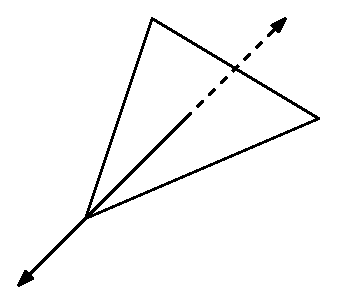
\includegraphics[scale=0.5]{src/geo/gfx/fig/pasch.eps}
\caption{\label{fig:pasch}Pasch's Axiom}
\end{center}
\end{figure}

\begin{lem}
Let \(\ell\) be a line and \(C \in \ell\) a point in an ordered geometry.
Suppose \(A\) and \(B\) are points not on \(\ell\) such that \(\BETWEEN{A}{B}{C}\).
Then \(A\) and \(B\) are on the same side of \(\ell\).
\end{lem}

\begin{proof}
Suppose otherwise that \(A\) and \(B\) are on opposite sides of \(\ell\).
By the Plane Separation property, and because \(A\) and \(B\) are not on \(\ell\), the segment \(\SEGMENT{A}{B}\) cuts \(\ell\) at a unique point \(D\).
That is, \(D \in \ell\) and \(\BETWEEN{A}{D}{B}\).
But note that \(C, D \in \ell\), so \(\LINE{C}{D} = \ell\), and also \(C, D \in \LINE{A}{B}\), so that \(\LINE{C}{D} = \LINE{A}{B}\).
But then \(\LINE{A}{B} = \ell\), a contradiction.
Thus \(A\) and \(B\) must be on the same side of \(\ell\).
\end{proof}

%---------%
\Exercises%
%---------%

    \newpage

  \section{Models of Ordered Geometry}
    To show that a given incidence geometry is an ordered geometry, we need to (1) specify how to detect when one point is between to others and (2) specify how to determine when two points are on the same side of a line.

\subsection{Betweenness in \(\RR^2\)}

\begin{prop}
The cartesian plane is an ordered geometry with 
\begin{proplist}
\item Given points \(A\), \(B\), and \(C\) in \(\RR^2\), we say \(\BETWEEN{A}{C}{B}\) if the equation \(C = A + t(B-A)\) has a solution \(t \in [0,1]\). This is a betweenness relation.
\item Given a line \(\ell = \LINE{A}{B}\), we define two half-planes as follows: \[ H_1 = \left\{ (x, y) \mid \DET \begin{bmatrix} a_x & a_y & 1 \\ b_x & b_y & 1 \\ x & y & 1 \end{bmatrix} > 0 \right\} \] and \[ H_2 = \left\{ (x, y) \mid \DET \begin{bmatrix} a_x & a_y & 1 \\ b_x & b_y & 1 \\ x & y & 1 \end{bmatrix} < 0 \right\}. \]
\end{proplist}
\end{prop}


\begin{itemize}
\item[B1.] Suppose \(\BETWEEN{A}{B}{A}\). Now \(B = A + t(A - A) = A\) as needed.
\item[B2.] Suppose \(A\), \(B\), and \(C\) are distinct points such that \(\BETWEEN{A}{C}{B}\). By definition, we have \(C = A + t(B-A)\) for some real number \(t \in [0,1]\). Certainly \(C \in \LINE{A}{B}\). Moreover, note that
\begin{eqnarray*}
B + (1-t)(A-B) & = & B + A - B - t(A-B) \\
 & = & A + t(B-A) \\
 & = & C,
\end{eqnarray*}
so that \(\BETWEEN{B}{C}{A}\).
\item[B3.] Suppose we have distinct points \(A\), \(B\), and \(C\) such that \(\BETWEEN{A}{B}{C}\) and \(\BETWEEN{B}{C}{A}\).
Now \(B = A + t(C-A)\) and \(C = B + u(A-B)\) for some real numbers \(u,t \in [0,1]\) by definition.
Substituting the second equation into the first, we see that \(B = A + t(1-u)(B - A)\), so that \(0 = (t(1-u) - 1)(B - A)\). Since \(A\) and \(B\) are distinct, we must have \(t(1-u) = 1\). Similarly, substituting the first equation into the second, we have \(u(1-t) = 1\). Then \(t\) must be a root of the quadratic \(t^2 - t + 1\), which has no real solutions.
\end{itemize}

We can say something a little stronger about the intersection of a segment and a line in \(\RR^2\); this next fact will become useful later, so we state and prove it now.

The Cartesian Plane has the Trichotomy Property, as we show. Let \(A\), \(B\), and \(C\) be distinct collinear points. Now \(C \in \LINE{A}{B}\), so that \(C = A + t(B-A)\) for some real number \(t\). If \(t \in [0,1]\), then \(\BETWEEN{A}{C}{B}\). If \(t > 1\), then \(\frac{1}{t} \in (0,1)\), and we have \(B = A + \frac{1}{t}(C-A)\) so that \(\BETWEEN{A}{B}{C}\). If \(t < 0\), then \(\frac{-t}{1-t} \in (0,1]\) and we have \(A = C + \frac{-t}{1-t}(B-C)\), so that \(\BETWEEN{C}{A}{B}\).

\begin{prop}
Let \(A,B \in \RR^2\) be distinct points and let \(X = (x_1, x_2), Y = (y_1, y_2) \in \RR^2\) be distinct points not in \(\ell_{A,B}\). Then \(\SEGMENT{X}{Y} \cap \LINE{A}{B}\) consists of a single point if and only if \[ \DET \begin{bmatrix} a_1 & a_2 & 1 \\ b_1 & b_2 & 1 \\ x_1 & x_2 & 1 \end{bmatrix} \quad \mathrm{and} \quad \DET \begin{bmatrix} a_1 & a_2 & 1 \\ b_1 & b_2 & 1 \\ y_1 & y_2 & 1 \end{bmatrix} \] have opposite signs.
\end{prop}

\begin{proof}
Note that \(\LINE{X}{Y} \cap \LINE{A}{B}\) contains exactly one point if and only if the equation \(X + t(Y-X) = A + u(B-A)\) has a unique solution \((t,u)\). In fact we have \[ \begin{bmatrix} t \\ -u \end{bmatrix} = \begin{bmatrix} y_1 - x_1 & b_1 - a_1 \\ y_2 - x_2 & b_2 - a_2 \end{bmatrix}^{-1} \begin{bmatrix} a_1 - x_1 \\ a_2 - x_2 \end{bmatrix}. \] Comparing entries of this matrix, we see that \[ t = \frac{(b_2-a_2)(a_1-x_1) + (a_1-b_1)(a_2-x_2)}{(y_1-x_1)(b_2-a_2) - (y_2-x_2)(b_1-a_1)}. \] Note that the unique point in \(\LINE{X}{Y} \cap \LINE{A}{B}\) is in fact in the segment \(\SEGMENT{X}{Y}\) if and only if \(t \in [0,1]\).

There are now two possibilities, depending on whether the denominator of \(t\) is positive or negative. If the denominator of \(t\) is positive, we can see that \(t \in (0,1)\) if and only if \[ \DET \begin{bmatrix} a_1 & a_2 & 1 \\ b_1 & b_2 & 1 \\ x_1 & x_2 & 1 \end{bmatrix} > 0 > \begin{bmatrix} a_1 & a_2 & 1 \\ b_1 & b_2 & 1 \\ y_1 & y_2 & 1 \end{bmatrix}. \] If the denominator of \(t\) is negative, then \(t \in (0,1)\) if and only if \[ \DET \begin{bmatrix} a_1 & a_2 & 1 \\ b_1 & b_2 & 1 \\ x_1 & x_2 & 1 \end{bmatrix} < 0 < \begin{bmatrix} a_1 & a_2 & 1 \\ b_1 & b_2 & 1 \\ y_1 & y_2 & 1 \end{bmatrix}. \qedhere \]
\end{proof}

Certainly both \(H_1\) and \(H_2\) are not empty, and they are disjoint by construction.

To see that \(H_1\) is convex, suppose BWOC that we have points \(X,Y \in H_1\) and a point \(Z = (z_1, z_2)\) such that \(\BETWEEN{X}{Z}{Y}\) and \(Z \notin H_1\). Now \[ m = \DET \begin{bmatrix} a_1 & a_2 & 1 \\ b_1 & b_2 & 1 \\ z_1 & z_2 & 1 \end{bmatrix} \] is either 0 or negative. If \(m = 0\), then in fact \(Z \in \LINE{A}{B}\). Since \(X,Y \notin \LINE{A}{B}\), we have that \(\SEGMENT{X}{Y}\) and \(\LINE{A}{B}\) meet at a single point \(Z\); but we've seen this can only happen if \(X \in H_1\) and \(Y \in H_2\) (or vice versa). Suppose instead that \(m < 0\); that is, \(Z \in H_2\). Now we have that \(\SEGMENT{X}{Z}\) and \(\SEGMENT{Y}{Z}\) each intersect \(\LINE{A}{B}\) at unique points, say \(W\) and \(V\), respectively. Note that \(\BETWEEN{X}{W}{Z}\) and \(\BETWEEN{Y}{V}{Z}\). Since \(\BETWEEN{X}{Z}{Y}\), we have that \(X\), \(Y\), \(Z\), \(W\), and \(V\) are all collinear. If \(W\) and \(V\) are distinct points, then in fact \(X, Y \in \LINE{W}{V} = \LINE{A}{B}\), a contradiction. If \(W = V\), then we have \(\BETWEEN{X}{W}{Z}\) and \(\BETWEEN{Y}{W}{Z}\), so by the 4-point axiom, \(\BETWEEN{W}{Z}{Y}\), a contradiction. So we must have \(Z \in H_1\), and thus \(H_1\) is convex. A similar argument shows that \(H_2\) is convex.

Finally, we need to show that if \(X \in H_1\) and \(Y \in H_2\), then \(\SEGMENT{X}{Y} \cap \LINE{A}{B}\) consists of a unique point. We showed precisely this previously.

    \newpage

  \section{Angles}
    \begin{dfn}[Angle]
Let $P$ be an ordered geometry and $x$, $o$, and $y$ distinct points. Then the set \[ \ANGLE{x}{o}{y} = \RAY{o}{x} \cup \RAY{o}{y} \] is called the \emph{angle}\index{angle} with \emph{vertex} $o$ and \emph{sides} $\RAY{o}{x}$ and $\RAY{o}{y}$. If $\BETWEEN{x}{o}{y}$, then we say the angle is \emph{straight}\index{angle!straight}, and if $\BETWEEN{o}{x}{y}$ or $\BETWEEN{o}{y}{x}$, then we say the angle is \emph{flat}\index{angle!flat}.
\begin{itemize}
\item Suppose $x$, $o$, and $y$ are not collinear. In this case, since $P$ is an ordered geometry, the lines $\LINE{o}{x}$ and $\LINE{o}{y}$ divide $P$ into half-planes. Let $H_1$ be the $y$ half-plane of $\LINE{o}{x}$, and let $K_1$ be the $x$ half-plane of $\LINE{o}{y}$. We define the \emph{interior} of $\ANGLE{x}{o}{y}$ to be the set \[ \INTANGLE{x}{o}{y} = H_1 \cap K_1. \] If $x$, $y$, and $o$ are collinear, then the interior of $\ANGLE{x}{o}{y}$ is not defined.
\end{itemize}
\end{dfn}

\begin{dfn}[Angle Pairs]
Suppose $x$, $y$, $z$, $w$, and $o$ are distinct points in an ordered geometry.
\begin{itemize}
\item $\ANGLE{x}{o}{y}$ and $\ANGLE{y}{o}{z}$ are called an \emph{adjacent pair}\index{angle!adjacent pair}.
\item $\ANGLE{x}{o}{y}$ and $\ANGLE{y}{o}{z}$ are called a \emph{linear pair}\index{angle!linear pair} if $\BETWEEN{x}{o}{z}$.
\item $\ANGLE{x}{o}{y}$ and $\ANGLE{z}{o}{w}$ are called a \emph{vertical pair}\index{angle!vertical pair} if $\BETWEEN{x}{o}{z}$ and $\BETWEEN{y}{o}{w}$.
\end{itemize}
\end{dfn}

\begin{thm}[Crossbar Theorem]
Suppose $O$, $A$, and $B$ are noncollinear points in an ordered geometry, and that $C \in \INTANGLE{A}{O}{B}$. Then $\RAY{O}{C}$ cuts $\SEGMENT{A}{B}$ at a unique point $D$.
\end{thm}

\begin{center}
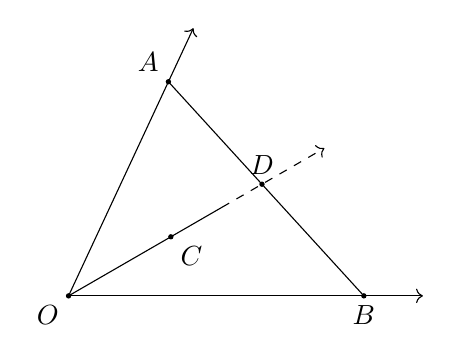
\begin{tikzpicture}[scale=1.5]
  \coordinate [label=below left:$O$] (O)   at (0  : 0);
  \coordinate [label=above left:$A$] (A)   at (65 : 2);
  \coordinate (A')  at (65 : 2.5);
  \coordinate [label=below:$B$]      (B)   at (0  : 2.5);
  \coordinate (B')  at (0  : 3);
  \coordinate (C)   at (30 : 1);
  \coordinate (C')  at (30 : 1.5);
  \coordinate (C'') at (30 : 2.5);

  \coordinate [label=above:$D$]      (D)   at (intersection of A--B and O--C'');

  \draw [->] (O) -- (A');
  \draw [->] (O) -- (B');

  \draw [fill] (O) circle [radius=0.5pt];
  \draw [fill] (A) circle [radius=0.5pt];
  \draw [fill] (B) circle [radius=0.5pt];

  \draw (O) -- (C');
  \draw [dashed, ->] (C') -- (C'');

  \draw [fill] (C) circle [radius=0.5pt];
  \node [below right] at (C) {$C$};

  \draw (A) -- (B);

  \draw [fill] (D) circle [radius=0.5pt];
\end{tikzpicture}
\end{center}

\begin{proof}
By the Interpolation property, there is a point $P$ on $\LINE{O}{A}$ such that $\BETWEEN{P}{O}{A}$. Note that $A$ and $P$ are on opposite sides of $\LINE{O}{B}$, so that $P$ and $C$ are on opposite sides of $\LINE{O}{B}$. (Since $A$ and $C$ are on the same side of $\LINE{O}{B}$ by definition.) Consider now the triangle $\TRIANGLE{P}{A}{B}$. Note that the line $\LINE{O}{C}$ does not contain $A$, $B$, or $P$, since $C$ is not on $\LINE{O}{A}$ or $\LINE{O}{B}$ by hypothesis. Moreover, $\LINE{O}{C}$ cuts $\SEGMENT{P}{A}$ at $O$. By Pasch's Axiom, $\LINE{O}{C}$ must also cut either $\SEGMENT{P}{B}$ or $\SEGMENT{A}{B}$.

Suppose $\LINE{O}{C}$ cuts $\SEGMENT{P}{B}$ at a (necessarily unique) point $Q$. Note that $\LINE{O}{C} = \LINE{Q}{C}$. Now $P$ and $Q$ are on the same side of $\LINE{O}{B}$, so that $Q$ and $C$ are on \emph{opposite} sides of $\LINE{O}{B}$. Thus, there is a unique point $R$ on $\LINE{O}{B}$ such that $\BETWEEN{Q}{R}{C}$. In particular, $R \in \LINE{O}{C}$. Now we have $O,R \in \LINE{O}{C}$ and $O, R \in \LINE{O}{B}$, so that $\LINE{O}{C} = \LINE{O}{B}$, a contradiction.

Hence $\LINE{O}{C}$ must cut $\SEGMENT{A}{B}$ at a unique point; say $D$. Now $D$ and $A$ are on the same side of $\LINE{O}{B}$, and so $C$ and $D$ are on the same side of $\LINE{O}{B}$; in particular, we cannot have $\BETWEEN{D}{O}{C}$. So in fact $\RAY{O}{C}$ cuts $\SEGMENT{A}{B}$ at a unique point.
\end{proof}


    \newpage

  \section{Congruence}
    Intuitively, we want to say that two sets of points in a geometry are ``congruent'' if they have the same size and shape. Rather than defining congruence once and for all, we will define congruence in terms of primitive congruence relations on two special kinds of sets: segments and angles.

\begin{dfn}[Segment Congruence]
Let \(P\) be an ordered geometry, and suppose we have an equivalence relation on pairs of points, denoted $\SEGCONG{\ast}{\ast}{\ast}{\ast}$. We call $\SEGCONG{\ast}{\ast}{\ast}{\ast}$ a \emph{segment congruence}\index{congruence!of segments} if the following properties are satisfied.
\begin{proplist}
\item[SC1.] $\SEGCONG{x}{x}{y}{y}$ for all points $x$ and $y$.
\item[SC2.] $\SEGCONG{x}{y}{y}{x}$ for all points $x$ and $y$.
\item[SC3.] If $z \in \RAY{x}{y}$ such that $\SEGCONG{x}{z}{x}{y}$, then $z = y$.
\end{proplist}
In this case, $\SEGCONG{\ast}{\ast}{\ast}{\ast}$ is well-defined on the set of \emph{segments} in $P$, where we write $\SEGMENT{x}{y} \equiv \SEGMENT{a}{b}$ to mean $\SEGCONG{x}{y}{a}{b}$.
\end{dfn}

The first property handles the ``trivial'' case, the second makes the relation well-defined on segments, and the third ensures that it differentiates between segments on the same ray which share an endpoint.

\begin{dfn}[Angle Congruence]
Let $P$ be an ordered geometry, and suppose we have an equivalence relation on triples of points, denoted $\ANGCONG{\ast}{\ast}{\ast}{\ast}{\ast}{\ast}$. We call $\ANGCONG{\ast}{\ast}{\ast}{\ast}{\ast}{\ast}$ an \emph{angle congruence}\index{congruence!of angles} if the following properties are satisfied.
\begin{itemize}
\item[AC1.] If $\BETWEEN{x}{y}{z}$ and $\BETWEEN{a}{b}{c}$, then $\ANGCONG{x}{y}{z}{a}{b}{c}$ and $\ANGCONG{y}{x}{z}{b}{a}{c}$, and it is not the case that $\ANGCONG{x}{y}{z}{y}{x}{z}$.
\item[AC2.] If $x \in \RAY{o}{a}$ and $y \in \RAY{o}{b}$ and $x$, $y$, and $o$ are distinct, then $\ANGCONG{a}{o}{b}{x}{o}{y}$.
\item[AC3.] $\ANGCONG{a}{o}{b}{b}{o}{a}$ for all points $a$, $o$, and $b$ with $a \neq o$ and $b \neq o$.
\item[AC4.] If $a$, $b$, and $o$ are noncollinear points and $x$ is on the $b$-side of $\LINE{o}{a}$ such that $\ANGCONG{a}{o}{b}{a}{o}{x}$, then $x \in \RAY{o}{b}$.
\end{itemize}
In this case, $\ANGCONG{\ast}{\ast}{\ast}{\ast}{\ast}{\ast}$ is an equivalence relation on the set of \emph{angles} in $P$, and we write $\ANGLE{a}{o}{b} \equiv \ANGLE{x}{p}{y}$ to mean $\ANGCONG{a}{o}{b}{x}{p}{y}$.
\end{dfn}

Much like the properties of segment congruence, the first property handles the trivial cases, the second and third make the relation well-defined on angles, and the fourth ensures that it differentiates between angles on one half-plane which share a vertex.

\begin{dfn}[Congruence Geometry]
Let $P$ be an ordered geometry. If $P$ has a segment congruence and an angle congruence, we say that $P$ is an \emph{ordered geometry}\index{ordered geometry}.
\end{dfn}

We can define congruence of many different kinds of figures in terms of segment and angle congruence. For instance...

\begin{dfn}[Triangle Congruence]
Let $a$, $b$, and $c$ be distinct points, and let $x$, $y$, and $z$ be distinct points. We say that $\TRIANGLE{a}{b}{c}$ is \emph{congruent}\index{congruence!of triangles} to $\TRIANGLE{x}{y}{z}$, denoted $\TRIANGLE{a}{b}{c} \equiv \TRIANGLE{x}{y}{z}$, if \[ \SEGMENT{a}{b} \equiv \SEGMENT{x}{y}, \quad \SEGMENT{b}{c} \equiv \SEGMENT{y}{z}, \quad \mathrm{and} \quad \SEGMENT{c}{a} \equiv \SEGMENT{z}{x} \] and \[ \ANGLE{a}{b}{c} \equiv \ANGLE{x}{y}{z}, \quad \ANGLE{b}{c}{a} \equiv \ANGLE{y}{z}{x}, \quad \mathrm{and} \quad \ANGLE{c}{a}{b} \equiv \ANGLE{z}{x}{y}. \]
\end{dfn}

\begin{dfn}
Let $a$, $b$, and $c$ be distinct points.
\begin{itemize}
\item We say that the triangle $\TRIANGLE{a}{b}{c}$ is \emph{equilateral}\index{equilateral} if $\SEGMENT{a}{b} \equiv \SEGMENT{b}{c} \equiv \SEGMENT{c}{a}$.
\item We say that the triangle $\TRIANGLE{a}{b}{c}$ is \emph{isoceles}\index{isoceles} if two of its sides are congruent to each other.
\end{itemize}
\end{dfn}


\begin{dfn}[Supplementary Angles]
We say that angles $\ANGLE{a}{o}{b}$ and $\ANGLE{x}{p}{y}$ are \emph{supplementary}\index{supplementary angles} if there is a linear pair, $\ANGLE{u}{q}{v}$ and $\ANGLE{v}{q}{w}$, such that $\ANGLE{a}{o}{b} \equiv \ANGLE{u}{q}{v}$ and $\ANGLE{x}{p}{y} \equiv \ANGLE{v}{q}{w}$. In this case we say that $\ANGLE{x}{p}{y}$ is a \emph{supplement} of $\ANGLE{a}{o}{b}$.
\end{dfn}

\begin{prop}
Let $P$ be an ordered geometry with an angle congruence.
\begin{proplist}
\item If two angles form a linear pair, then they are supplementary.
\item Every angle has a supplement.
\end{proplist}
\end{prop}

\begin{dfn}
An angle is called \emph{right} if it is supplementary to itself.
\end{dfn}


%---------%
\Exercises%
%---------%

\begin{exercise}
Show that triangle congruence is an equivalence relation.
\end{exercise}

    \newpage

  \section{Models of Congruence Geometry}
    Remember: to show that an ordered geometry is a congruence geometry, we need to specify (1) how to detect when two segments are congruent and (2) how to detect when two angles are congruent.

\subsection{Congruence in \(\RR^2\)}

\begin{prop}
Define a map \(\delta : \RR^2 \times \RR^2 \rightarrow \RR\) by \(\delta(A,B) = (B-A) \cdot (B-A)\), where \(\cdot\) denotes the usual dot product.
Now \(\RR^2\) is a congruence geometry under the following relations.
\begin{proplist}
\item Given points \(A\), \(B\), \(X\), and \(Y\) in \(\RR^2\), we say that \(\SEGCONG{A}{B}{X}{Y}\) if \[ \delta(A,B) = \delta(X,Y). \]
\item Given points \(A\), \(O\), \(B\), \(X\), \(P\), and \(Y\) in \(\RR^2\) such that \(A \neq O\), \(B \neq O\), \(X \neq P\), and \(Y \neq P\), we say that \(\ANGCONG{A}{O}{B}{X}{P}{Y}\) if \[ \frac{((A-O) \cdot (B-O))^2}{\delta(A,O)\delta(B,O)} = \frac{((X-P) \cdot (Y-P))^2}{\delta(X,P)\delta(Y,P)}. \]
\end{proplist}
\end{prop}

\begin{proof}
(@@@)
\end{proof}



\subsection{Congruence in the Unit Disc}



    \newpage

  \section{Circles}
    \begin{dfn}[Circle]
Let $P$ be a congruence geometry and let $o,a \in P$ be points.
The set \[ \CIRCLE{o}{a} = \{ x \in P \mid \SEGMENT{o}{x} \equiv \SEGMENT{o}{a} \} \] is called the \emph{circle}\index{circle} with \emph{center} $o$ and \emph{passing through} $a$.
\end{dfn}


\begin{dfn}[Radius, Diameter, Chord]
(@@@)
\end{dfn}

    \newpage

  \section{Plane Geometry}
    \begin{dfn}[Plane Geometry]
Let \(P\) be an ordered geometry with a segment congruence and an angle congruence.
We say that \(P\) is a \emph{plane geometry} if the following properties are satisfied.
\begin{proplist}
\item \textbf{Right Angle Property.} Any two right angles are congruent.

\item \textbf{Circle-Ray Cut.} If \(o\), \(a\), and \(b\) are points such that \(a \neq o\) and \(b \neq o\), then there is a unique point \(c \in \RAY{o}{b}\) such that \(\SEGMENT{o}{c} \equiv \SEGMENT{o}{a}\).

\begin{center}
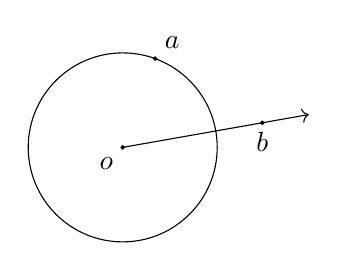
\begin{tikzpicture}[scale=0.6]
  \coordinate [label=below left:\(o\)]  (o) at (0  : 0);
  \draw [fill] (o) circle [radius=1pt];
  \coordinate [label=above right:\(a\)] (a) at (70 : 2);
  \draw [fill] (a) circle [radius=1pt];
  \coordinate [label=below:\(b\)]       (b) at (10 : 3);
  \draw [fill] (b) circle [radius=1pt];
  \draw [->] (o) -- (10: 4);
  \draw (o) circle [radius=2];
\end{tikzpicture}
\end{center}

\item \textbf{Circle-Circle Cut.} Let \(o\), \(a\), \(P\), and \(x\) be points, and suppose there are distinct points \(u\) and \(v\) on \(\CIRCLE{p}{x}\) such that \(u \in \INTCIRCLE{o}{a}\) and \(v \in \EXTCIRCLE{o}{a}\).
Then \(\CIRCLE{o}{a} \cap \CIRCLE{p}{x}\) contains two distinct points.

\begin{center}
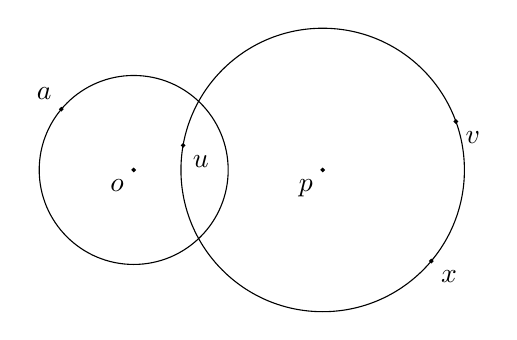
\begin{tikzpicture}[scale=0.6]
  \coordinate [label=below left:{\(o\)}]  (o) at (0,0);
  \draw [fill] (o) circle [radius=1pt];
  \coordinate [label=above left:{\(a\)}] (a) at ($ (o)+(140 : 2) $);
  \draw [fill] (a) circle [radius=1pt];
  \draw (o) circle [radius=2];
  \coordinate [label=below left:\(p\)]  (p) at (4,0);
  \draw [fill] (p) circle [radius=1pt];
  \coordinate [label=below right:\(x\)] (x) at ($ (p)+(320 : 3) $);
  \draw [fill] (x) circle [radius=1pt];
  \coordinate [label=below right:\(u\)] (u) at ($ (p)+(170 : 3) $);
  \draw [fill] (u) circle [radius=1pt];
  \coordinate [label=below right:\(v\)] (v) at ($ (p)+(20  : 3) $);
  \draw [fill] (v) circle [radius=1pt];
  \draw (p) circle [radius=3];
\end{tikzpicture}
\end{center}

\item \textbf{Circle Cut Transfer.} Suppose \(a\), \(b\), \(c\), \(d\), \(x\), \(y\), \(z\), and \(w\) are points such that \(\SEGMENT{a}{b} \equiv \SEGMENT{x}{y}\), \(\SEGMENT{b}{c} \equiv \SEGMENT{y}{z}\), and \(\SEGMENT{c}{d} \equiv \SEGMENT{z}{w}\).
If \(\CIRCLE{b}{a} \cap \CIRCLE{c}{d}\) is not empty, then \(\CIRCLE{y}{x} \cap \CIRCLE{z}{w}\) is not empty.

\item \textbf{Angle-Side Congruence.} Suppose \(a\), \(b\), \(c\), \(x\), \(y\), and \(z\) are points such that \(\SEGMENT{b}{a} \equiv \SEGMENT{y}{x}\) and \(\SEGMENT{b}{c} \equiv \SEGMENT{y}{z}\).
Then \(\SEGMENT{a}{c} \equiv \SEGMENT{x}{z}\) if and only if \(\ANGLE{a}{b}{c} \equiv \ANGLE{x}{y}{z}\).
\end{proplist}
\end{dfn}

The Circle Separation and Circle Cut properties allow us to construct points on the intersection of a circle with a central ray and of two circles, respectively.
(Without these we have no way to construct points on circles!)
The Circle Cut Transfer property says that our geometry is ``uniform'' in some sense, allowing us to shift points in the intersection of two circles.
Angle-Side Congruence provides an essential link between segment congruence and angle congruence, which are otherwise unrelated.


In the remainder of this section, suppose \(P\) is a plane geometry.

\begin{prop}[Circle Trichotomy]
Let \(o\) and \(a\) be distinct points.
Then \(\CIRCLE{o}{a}\), \(\INTCIRCLE{o}{a}\), and \(\EXTCIRCLE{o}{a}\) partition the set of points in \(P\).
That is, every point is either on \(\CIRCLE{o}{a}\), interior to \(\CIRCLE{o}{a}\), or exterior to \(\CIRCLE{o}{a}\).
\end{prop}

\begin{prop}[SSS Theorem]
If two triangles can be labeled such that corresponding sides are congruent, then the triangles are congruent.
More precisely, let \(a\), \(b\), and \(c\) be distinct points and \(x\), \(y\), and \(z\) be distinct points.
If \(\SEGMENT{a}{b} \equiv \SEGMENT{x}{y}\), \(\SEGMENT{b}{c} \equiv \SEGMENT{y}{z}\), and \(\SEGMENT{c}{a} \equiv \SEGMENT{z}{x}\), then \(\TRIANGLE{a}{b}{c} \equiv \TRIANGLE{x}{y}{z}\).
\end{prop}

\begin{proof}
That \(\ANGLE{a}{b}{c} \equiv \ANGLE{x}{y}{z}\), \(\ANGLE{b}{c}{a} \equiv \ANGLE{y}{z}{x}\), and \(\ANGLE{z}{x}{y} \equiv \ANGLE{c}{a}{b}\) follows from three applications of the Angle-Side Congruence property.
\end{proof}

\begin{prop}[Uniqueness of Circle Cuts]
Let \(o\), \(a\), \(P\), \(x\), and \(h\) be points, with \(o\) and \(P\) distinct and with \(h\) not on \(\LINE{o}{p}\).
There is at most one point \(u \in \CIRCLE{o}{a} \cap \CIRCLE{p}{x}\) on the \(h\)-side of \(\LINE{o}{p}\).
\end{prop}

\begin{proof}
Suppose we have two such points, \(u\) and \(v\).
That is, both \(u\) and \(v\) are on the \(h\)-side of \(\LINE{o}{p}\) and \(u,v \in \CIRCLE{o}{a} \cap \CIRCLE{p}{x}\).
Note that \(\SEGMENT{o}{p} \equiv \SEGMENT{o}{p}\), \(\SEGMENT{p}{u} \equiv \SEGMENT{p}{x} \equiv \SEGMENT{p}{v}\), and \(\SEGMENT{u}{o} \equiv \SEGMENT{a}{o} \equiv \SEGMENT{v}{o}\).
By the SSS Theorem, we have \(\TRIANGLE{u}{o}{p} \equiv \TRIANGLE{v}{o}{p}\).
In particular, we have \(\ANGLE{u}{o}{p} \equiv \ANGLE{v}{o}{p}\) and \(\ANGLE{u}{p}{o} \equiv \ANGLE{v}{p}{o}\).
Now by AC7, we have \(v \in \RAY{o}{u} \subseteq \LINE{o}{u}\) and \(u \in \RAY{p}{v} \subseteq \LINE{p}{v}\).
That is, \(u\) and \(v\) are points in the intersection of the lines \(\LINE{o}{u}\) and \(\LINE{p}{v}\).
Since \(o\) and \(P\) are distinct, these lines must be distinct, and so they intersect at a unique point.
Hence \(u = v\).
\end{proof}

\begin{prop}[SAS Theorem]
If two triangles can be labeled such that two corresponding sides, and the angles between, are congruent, then the triangles are congruent.
More precisely, let \(a\), \(b\), and \(c\) be distinct points, and \(x\), \(y\), and \(z\) be distinct points.
If \(\SEGMENT{a}{b} \equiv \SEGMENT{x}{y}\), \(\SEGMENT{b}{c} \equiv \SEGMENT{y}{z}\), and \(\ANGLE{a}{b}{c} \equiv \ANGLE{x}{y}{z}\), then \(\TRIANGLE{a}{b}{c} \equiv \TRIANGLE{x}{y}{z}\).
\end{prop}

\begin{prop}[Pons Asinorum (Bridge of Asses)]
If \(\TRIANGLE{a}{b}{c}\) is isoceles with \(\SEGMENT{a}{b} \equiv \SEGMENT{b}{c}\), then \(\ANGLE{b}{a}{c} \equiv \ANGLE{b}{c}{a}\).
\end{prop}

\begin{proof}
We have two triangles, \(\TRIANGLE{b}{a}{c}\) and \(\TRIANGLE{b}{c}{a}\), such that \(\SEGMENT{b}{c}\equiv \SEGMENT{b}{a}\), \(\SEGMENT{b}{a} \equiv \SEGMENT{b}{c}\), and \(\ANGLE{c}{b}{a} \equiv \SEGMENT{a}{b}{c}\).
By the SAS Theorem, \(\TRIANGLE{b}{a}{c} \equiv \SEGMENT{b}{c}{a}\), and thus \(\ANGLE{b}{a}{c} \equiv \ANGLE{b}{c}{a}\).
\end{proof}

\begin{cor}
Every triangle which is equilateral is also equiangular; all three interior angles are congruent.
\end{cor}

\begin{construct}[equilateral triangle with a given side]
Given distinct points \(x\) and \(y\), there exist points \(z_1\) and \(z_2\), on opposite sides of \(\LINE{x}{y}\), such that \(\TRIANGLE{x}{y}{z_1}\) and \(\TRIANGLE{x}{y}{z_2}\) are equilateral.
In fact, we have \(\TRIANGLE{x}{y}{z_1} \equiv \TRIANGLE{x}{y}{z_2}\).
\end{construct}

\begin{proof}
Consider the line \(\LINE{x}{y}\).
By the Interpolation property, there exists a point \(u\) such that \(\BETWEEN{u}{x}{y}\).
By the Circle Separation property, there is a point \(w \in \CIRCLE{y}{x} \cap \RAY{x}{w}\).
Note in particular that \(\BETWEEN{w}{x}{y}\), and hence \(w\) is exterior to the circle \(\CIRCLE{y}{x}\).
Moreover, \(w\) is on \(\CIRCLE{x}{y}\).
Now \(y\) is also on \(\CIRCLE{x}{y}\), and by definition, \(y\) is interior to \(\CIRCLE{y}{x}\).
By the Circle Cut property, there exist two points in \(\CIRCLE{x}{y} \cap \CIRCLE{y}{x}\), say \(z_1\) and \(z_2\), which must be on opposite sides of \(\LINE{x}{y}\) by the uniqueness of circle cuts.
Now \(\SEGMENT{x}{z_1} \equiv \SEGMENT{x}{y} \equiv \SEGMENT{y}{z_1}\) and \(\SEGMENT{x}{z_2} \equiv \SEGMENT{x}{y} \equiv \SEGMENT{y}{z_2}\) by the definition of circles, so that \(\TRIANGLE{x}{y}{z_1}\) and \(\TRIANGLE{x}{y}{z_2}\) are equilateral by definition.
Moreover, \(\TRIANGLE{x}{y}{z_1} \equiv \TRIANGLE{x}{y}{z_2}\) by the transitivity of segment congruence and the SSS Theorem.
\end{proof}

\begin{prop}[Segment Addition Theorem]
Suppose \(\BETWEEN{a}{b}{c}\) and \(\BETWEEN{x}{y}{z}\).
If any two of \(\SEGMENT{a}{b} \equiv \SEGMENT{x}{y}\), \(\SEGMENT{b}{c} \equiv \SEGMENT{y}{z}\), and \(\SEGMENT{a}{c} \equiv \SEGMENT{x}{z}\) hold, then so does the third.
\end{prop}

\begin{proof}
Note that \(\ANGLE{a}{b}{c} \equiv \ANGLE{x}{y}{z}\), \(\ANGLE{b}{c}{a} \equiv \ANGLE{y}{z}{x}\), and \(\ANGLE{c}{a}{b} \equiv \ANGLE{z}{x}{y}\) by AC4.
The result then follows from the SAS Theorem.
\end{proof}

\begin{lem}
Suppose \(\BETWEEN{a}{b}{c}\) and \(y \in \RAY{x}{z}\).
If \(\SEGMENT{a}{b} \equiv \SEGMENT{x}{y}\) and \(\SEGMENT{a}{c} \equiv \SEGMENT{x}{z}\), then \(\BETWEEN{x}{y}{z}\).
\end{lem}

\begin{proof}
Since \(y \in \RAY{x}{z}\), we have four possibilities: \(y = x\), \(\BETWEEN{x}{y}{z}\), \(y = z\), and \(\BETWEEN{x}{z}{y}\).
If \(y = x\), then we have \(\SEGMENT{a}{b} \equiv \SEGMENT{x}{x}\), so that \(b = a\), a contradiction.
Similarly if \(y = z\) then we have \(\SEGMENT{x}{y} \equiv \SEGMENT{x}{z}\), so that \(y = z\), also a contradiction.
Now suppose that \(\BETWEEN{x}{z}{y}\).
Note that \(\ANGLE{c}{a}{b} \equiv \ANGLE{z}{x}{y}\), \(\SEGMENT{a}{c} \equiv \SEGMENT{x}{z}\), and \(\SEGMENT{a}{b} \equiv \SEGMENT{x}{y}\); by the SAS Theorem, \(\TRIANGLE{a}{b}{c} \equiv \TRIANGLE{x}{y}{z}\).
In particular, the flat angle \(\ANGLE{a}{c}{b}\) is congruent to the straight angle \(\ANGLE{x}{z}{y}\), a contradiction.
Thus \(\BETWEEN{x}{y}{z}\) as claimed.
\end{proof}

\begin{construct}[copy a segment onto a ray]
Let \(a\) and \(b\) be distinct points, and let \(o\) and \(t\) be distinct points.
There exists a point \(x\) on \(\RAY{o}{t}\) such that \(\SEGMENT{o}{x} \equiv \SEGMENT{a}{b}\).
\end{construct}

\begin{proof}
First we construct a point \(z\) such that \(\TRIANGLE{a}{o}{z}\) is equilateral; now \(\SEGMENT{z}{a} \equiv \SEGMENT{z}{o}\).
Using the Interpolation property, construct a point \(h\) such that \(\BETWEEN{z}{a}{h}\), and using the Circle Separation property, construct a point \(u\) on \(\RAY{a}{h}\) such that \(\SEGMENT{a}{u} \equiv \SEGMENT{a}{b}\).
Again using Circle Separation, construct a point \(v\) on \(\RAY{z}{o}\) such that \(\SEGMENT{z}{v} \equiv \SEGMENT{z}{u}\).
By the previous proposition, \(\BETWEEN{z}{o}{v}\).
Now \(\SEGMENT{z}{a} \equiv \SEGMENT{z}{o}\) and \(\SEGMENT{z}{u} \equiv \SEGMENT{z}{v}\), thus \(\SEGMENT{a}{u} \equiv \SEGMENT{o}{v}\).
Again using Circle Separation, construct a point \(x\) on \(\RAY{o}{t}\) such that \(\SEGMENT{o}{x} \equiv \SEGMENT{o}{v}\).
Then we have \(\SEGMENT{o}{x} \equiv \SEGMENT{o}{v} \equiv \SEGMENT{a}{u} \equiv \SEGMENT{a}{b}\) as needed.
\end{proof}

\begin{construct}[copy an angle onto a ray]
Let \(a\), \(o\), \(b\) be distinct noncollinear points and let \(P\) and \(x\) be distinct points.
There exist two points \(y_1\) and \(y_2\), on opposite sides of \(\LINE{p}{x}\), such that \(\ANGLE{x}{p}{y_1} \equiv \ANGLE{x}{p}{y_2} \equiv \ANGLE{a}{o}{b}\). 
\end{construct}

\begin{proof}
First copy segment \(\SEGMENT{o}{b}\) onto \(\RAY{p}{x}\) at the point \(u\), then copy the segment \(\SEGMENT{b}{a}\) onto the ray \(\RAY{u}{p}\) at the point \(v\).
Now copy \(\SEGMENT{o}{a}\) onto \(\RAY{p}{x}\) at the point \(w\).
Note that \(\SEGMENT{o}{a} \equiv \SEGMENT{p}{w}\), \(\SEGMENT{o}{b} \equiv \SEGMENT{p}{u}\), and \(\SEGMENT{b}{a} \equiv \SEGMENT{u}{v}\).
Moreover, the intersection \(\CIRCLE{o}{a} \cap \CIRCLE{b}{a}\) is nonempty, as it contains \(a\).
By the Circle Cut Transfer property, \(\CIRCLE{p}{w} \cap \CIRCLE{u}{v}\) contains two points \(z_1\) and \(z_2\) on opposite sides of \(\LINE{p}{x}\).
By the SSS Theorem, we have \(\TRIANGLE{p}{u}{z_1} \equiv \TRIANGLE{o}{b}{a} \equiv \TRIANGLE{p}{u}{z_2}\), and thus \(\ANGLE{u}{p}{z_1} \equiv \ANGLE{a}{o}{b} \equiv \ANGLE{u}{p}{z_2}\) as needed.
\end{proof}

\begin{prop}[ASA Theorem]
Let \(a\), \(b\), \(c\) be distinct noncollinear points, and let \(x\), \(y\), \(z\) be distinct points.
If \(\ANGLE{a}{b}{c} \equiv \ANGLE{x}{y}{z}\), \(\SEGMENT{b}{c} \equiv \SEGMENT{y}{z}\), and \(\ANGLE{b}{c}{a} \equiv \ANGLE{y}{z}{x}\), then \(\TRIANGLE{a}{b}{c} \equiv \TRIANGLE{x}{y}{z}\).
\end{prop}

\begin{proof}
Copy \(\SEGMENT{y}{x}\) onto \(\RAY{b}{a}\) at \(d\).
Note that \(d\) and \(a\) are on the same side of \(\LINE{b}{c}\).
Moreover, we have \(\TRIANGLE{d}{b}{c} \equiv \TRIANGLE{x}{y}{z}\) by the SAS Theorem, and so \(\ANGLE{b}{c}{d} \equiv \ANGLE{y}{z}{x} \equiv \ANGLE{b}{c}{a}\).
By AC7, we have \(d \in \RAY{c}{a}\).
Now \(d\) is on both \(\LINE{b}{a}\) and \(\LINE{c}{a}\), and since \(a\), \(b\), and \(c\) are not collinear, we must have \(d = a\).
So \(\TRIANGLE{a}{b}{c} \equiv \TRIANGLE{x}{y}{z}\) as claimed.
\end{proof}

\begin{prop}[Angle Addition Theorem]
Suppose \(B \in \INTANGLE{A}{O}{C}\) and \(Y \in \INTANGLE{X}{P}{Z}\).
If any two of \(\ANGLE{A}{O}{C} \equiv \ANGLE{X}{P}{Z}\), \(\ANGLE{A}{O}{B} \equiv \ANGLE{X}{P}{Y}\), and \(\ANGLE{B}{O}{C} \equiv \ANGLE{Y}{P}{Z}\) holds, then so does the third.
\end{prop}

\begin{proof}
(@@@ Uses SAS and segment addition.)
\end{proof}

    \newpage

  \section{Transversals}
    \begin{prop}[Supplements are unique] \mbox{}
\begin{itemize}
\item Suppose that \(\ANGLE{A}{O}{B}\) and \(\ANGLE{B}{O}{C}\) are a linear pair, and that \(\ANGLE{X}{P}{Y}\) and \(\ANGLE{Y}{P}{Z}\) are a linear pair.
If \(\ANGLE{A}{O}{B} \equiv \ANGLE{X}{P}{Y}\), then \(\ANGLE{B}{O}{C} \equiv \ANGLE{Y}{P}{Z}\).
\item Suppose \(\ANGLE{A}{B}{C}\) and \(\ANGLE{X}{Y}{Z}\) are supplementary, and that \(\ANGLE{A}{B}{C}\) and \(\ANGLE{H}{K}{L}\) are supplementary.
Then \(\ANGLE{X}{Y}{Z} \equiv \ANGLE{H}{K}{L}\).
\end{itemize}
\end{prop}

\begin{proof}
Suppose we have two such linear pairs.
Without loss of generality, we can suppose that \[ \SEGMENT{O}{A} \equiv \SEGMENT{O}{B} \equiv \SEGMENT{O}{C} \equiv \SEGMENT{P}{X} \equiv \SEGMENT{P}{Y} \equiv \SEGMENT{P}{Z}. \] (If they aren't, we can use Circle Separation and the Segment Copy construction to find such points.) Now \(\TRIANGLE{B}{O}{A} \equiv \TRIANGLE{Y}{P}{X}\) by SAS, so that \(\ANGLE{B}{A}{O} \equiv \ANGLE{Y}{X}{P}\).
Now \(\SEGMENT{A}{C} \equiv \SEGMENT{X}{Z}\), so that \(\TRIANGLE{B}{A}{C} \equiv \TRIANGLE{Y}{X}{Z}\) by SAS.
So \(\SEGMENT{B}{C} \equiv \SEGMENT{Y}{Z}\), and thus \(\TRIANGLE{B}{O}{C} \equiv \TRIANGLE{Y}{P}{Z}\) by SSS.
Thus \(\ANGLE{B}{O}{C} \equiv \ANGLE{Y}{P}{Z}\).

The second statement follows easily.
\end{proof}

\begin{cor}
Vertical pairs of angles are congruent.
\end{cor}


\begin{dfn}[Transversal]
Suppose we have three lines \(\ell_1\), \(\ell_2\), and \(t\) in a plane geometry.
We say that \(t\) is a \emph{transversal} of \(\ell_1\) and \(\ell_2\) if \(t\) cuts both \(\ell_1\) and \(\ell_2\) at unique points, and these points are distinct.
\end{dfn}

Suppose \(t\) is a transversal of \(\ell_1\) and \(\ell_2\), cutting these lines at \(O_1\) and \(O_2\), respectively as shown.

\begin{center}
\begin{tikzpicture}[scale=0.6]
  \coordinate (x1) at (-5,0);
  \coordinate (y1) at (4,0);
  \draw [<->] (x1) -- (y1);
  \node at (4,-0.5) {\(\ell_1\)};
  \coordinate (x2) at (-4,5);
  \coordinate (y2) at (4,3);
  \draw [<->] (x2) -- (y2);
  \node  at (-3,5.5) {\(\ell_2\)};
  \coordinate (x3) at (-1,-1);
  \coordinate (y3) at (1,6);
  \draw [<->] (x3) -- (y3);
  \node at (0.7,6) {\(t\)};
  \coordinate [label=below right:\(O_1\)] (o1) at (intersection of x1--y1 and x3--y3);
  \draw [fill] (o1) circle [radius=1pt];
  \coordinate [label=below left:\(O_2\)] (o2) at (intersection of x2--y2 and x3--y3);
  \draw [fill] (o2) circle [radius=1pt];
  \coordinate (x4) at (-0.5,2);
  \coordinate (y4) at (1,3);
  \coordinate [label=below:\(A\)] (a) at (intersection of x1--y1 and x4--y4);
  \draw [fill] (a) circle [radius=1pt];
  \coordinate [label=below:\(B\)] (b) at (intersection of x2--y2 and x4--y4);
  \draw [fill] (b) circle [radius=1pt];
\end{tikzpicture}
\end{center}

If \(A\) is on \(\ell_1\) and \(B\) is on \(\ell_2\) such that \(A\) and \(B\) are on opposite sides of \(t\), then we say that \(\ANGLE{A}{O_1}{O_2}\) and \(\ANGLE{B}{O_2}{O_1}\) are \emph{alternate interior angles} of this transversal.

\begin{prop}[Alternate Interior Angles]
If two lines \(\ell_1\) and \(\ell_2\) are cut by a transversal \(t\) so that a pair of alternate interior angles are congruent, then \(\ell_1\) and \(\ell_2\) are parallel.
\end{prop}

\begin{proof}
Suppose \(t\) meets \(\ell_1\) and \(\ell_2\) at points \(O_1\) and \(O_2\) respectively, and that \(A\) and \(B\) are on \(\ell_1\) and \(\ell_2\), respectively, and on opposite sides of \(t\).
Let \(C\) be on \(\ell_1\) such that \(\BETWEEN{A}{O_1}{C}\).
Suppose by way of contradiction that \(\ell_1\) and \(\ell_2\) are \emph{not} parallel; rather, they meet at a point \(X\) which (WLOG) is on the \(A\)-side of \(t\).
Copy \(\SEGMENT{O_1}{X}\) onto \(\RAY{O_2}{B}\) at the point \(Y\).
Now \(\SEGMENT{O_1}{X} \equiv \SEGMENT{O_2}{Y}\), \(\SEGMENT{O_1}{O_2} \equiv \SEGMENT{O_2}{O_1}\), and \(\ANGLE{X}{O_1}{O_2} \equiv \ANGLE{Y}{O_2}{O_1}\), so by SAS we have \(\TRIANGLE{X}{O_1}{O_2} \equiv \TRIANGLE{Y}{O_2}{O_1}\).
In particular, \(\ANGLE{O_2}{O_1}{Y} \equiv \ANGLE{O_1}{O_2}{X}\).

Now \(\ANGLE{X}{O_2}{O_1}\) and \(\ANGLE{O_1}{O_2}{Y}\) are supplementary, and \(\ANGLE{O_1}{O_2}{Y} \equiv \ANGLE{A}{O_1}{O_2}\), so that \(\ANGLE{A}{O_1}{O_2}\) and \(\ANGLE{X}{O_2}{O_1}\) are supplementary.
Since \(\ANGLE{X}{O_2}{O_1} \equiv \ANGLE{Y}{O_1}{O_2}\), we have that \(\ANGLE{A}{O_1}{O_2}\) and \(\ANGLE{Y}{O_1}{O_2}\) are supplementary.
But also \(\ANGLE{A}{O_1}{O_2}\) and \(\ANGLE{O_2}{O_1}{C}\) are supplementary.
Now \(\ANGLE{O_2}{O_1}{Y} \equiv \ANGLE{O_2}{O_1}{C}\).
By the uniqueness of congruent angles on a half-plane, we have that \(O_1\), \(C\), and \(Y\) are collinear, so that \(Y \in \ell_1\).
But now \(\ell_1\) and \(ell_2\) have two points in common -- \(X\) and \(Y\) -- and thus must be equal, a contradiction.

So in fact \(\ell_1\) and \(\ell_2\) must be parallel. 
\end{proof}

\begin{prop}[AAS]
Suppose we have triangles \(\TRIANGLE{A}{B}{C}\) and \(\TRIANGLE{X}{Y}{Z}\) such that \(\ANGLE{C}{A}{B} \equiv \ANGLE{Z}{X}{Y}\), \(\ANGLE{A}{B}{C} \equiv \ANGLE{X}{Y}{Z}\), and \(\SEGMENT{B}{C} \equiv \SEGMENT{Y}{Z}\).
Then \(\TRIANGLE{A}{B}{C} \equiv \TRIANGLE{X}{Y}{Z}\).
\end{prop}

\begin{proof}
Copy \(\SEGMENT{B}{A}\) onto \(\RAY{Y}{X}\) at the point \(W\).
Note that \(\TRIANGLE{W}{Y}{Z} \equiv \TRIANGLE{A}{B}{C}\) by SAS, so that \(\ANGLE{B}{A}{C} \equiv \TRIANGLE{Y}{W}{Z}\).
Suppose now that \(W\) and \(X\) are distinct points.
In this case \(\LINE{X}{Z}\) and \(\LINE{W}{Z}\) are lines cut by a transversal \(\LINE{X}{Y}\).
Moreover, if we let \(U\) be a point such that \(\BETWEEN{U}{X}{Z}\), then \(\ANGLE{U}{X}{W}\) and \(\ANGLE{Y}{X}{Z}\) are vertical, hence congruent, and so \(\ANGLE{U}{X}{W} \equiv \ANGLE{Y}{X}{Z}\).
But now by the Alternate Interior Angles theorem \(\LINE{X}{Z}\) and \(\LINE{W}{Z}\) must be parallel, a contradiction since they meet at \(Z\).
So in fact \(X\) and \(W\) are the same point, and thus \(\TRIANGLE{A}{B}{C} \equiv \TRIANGLE{X}{Y}{Z}\) by SAS.
\end{proof}

\begin{prop}[HL]
Let \(\TRIANGLE{A}{B}{C}\) and \(\TRIANGLE{X}{Y}{Z}\) be triangles such that \(\ANGLE{B}{C}{A}\) and \(\ANGLE{Y}{Z}{X}\) are right and \(\SEGMENT{A}{B} \equiv \SEGMENT{X}{Y}\) and \(\SEGMENT{B}{C} \equiv \SEGMENT{Y}{Z}\).
Then \(\TRIANGLE{A}{B}{C} \equiv \TRIANGLE{X}{Y}{Z}\).
\end{prop}

\begin{proof}
Copy \(\SEGMENT{Z}{X}\) onto the ray opposite \(\RAY{C}{A}\) at the point \(D\).
Now \(\ANGLE{B}{C}{D}\) is a right angle, since it is supplementary to \(\ANGLE{A}{C}{B}\).
By SAS, we have \(\TRIANGLE{X}{Y}{Z} \equiv \TRIANGLE{D}{C}{B}\), and thus \(\SEGMENT{B}{D} \equiv \SEGMENT{Y}{X} \equiv \SEGMENT{B}{A}\).
Now \(\TRIANGLE{A}{B}{D}\) is isoceles with \(\SEGMENT{B}{A} \equiv \SEGMENT{B}{D}\), so that \(\ANGLE{B}{A}{C} \equiv \ANGLE{B}{A}{D} \equiv \ANGLE{B}{D}{A} \equiv \ANGLE{Y}{X}{Z}\).
By AAS, we have \(\TRIANGLE{A}{B}{C} \equiv \TRIANGLE{X}{Y}{Z}\).
\end{proof}

\begin{prop}
A triangle formed by three noncollinear points cannot have two interior angles which are both right.
\end{prop}

\begin{proof}
Such a triangle would violate the Alternate Interior Angles theorem since right angles are self-supplementary, and any two right angles are congruent.
\end{proof}


\begin{construct}[Angle Bisector]
Let \(A\), \(O\), and \(B\) be noncollinear points.
There exists a unique line \(\ell\), containing \(O\), such that if \(U \in \ell\) is different from \(O\) then \(\ANGLE{A}{O}{U} \equiv \ANGLE{B}{O}{U}\).
This line is called the \emph{bisector} of \(\ANGLE{A}{O}{B}\).
\end{construct}

\begin{proof}
Note that we can assume WLOG that \(\SEGMENT{O}{A} \equiv \SEGMENT{O}{B}\); if not, construct such a point on \(\RAY{O}{B}\) using the Circle Separation property.
Since the intersection of \(\CIRCLE{A}{O}\) and \(\CIRCLE{B}{O}\) contains a point not on \(\LINE{A}{B}\), by Circle Cut Transfer there is a second point \(U\) on the opposite side of \(\LINE{A}{B}\) such that \(\SEGMENT{A}{U} \equiv \SEGMENT{B}{U}\).
Let \(\ell = \LINE{O}{U}\).
Note that \(\TRIANGLE{A}{O}{U} \equiv \TRIANGLE{B}{O}{U}\) by SSS, so that \(\ANGLE{A}{O}{U} \equiv \ANGLE{B}{O}{U}\).
Then if \(V\) is a point such that \(\BETWEEN{V}{O}{U}\), we have \(\ANGLE{V}{O}{A} \equiv \ANGLE{V}{O}{B}\), since these are supplementary to congruent angles.

To see uniqueness, note that any such line must contain \(O\) and \(U\).
\end{proof}

\begin{cor}
\(A\) and \(B\) are on opposite sides of the bisector of \(\ANGLE{A}{O}{B}\).
In particular, the bisector of \(\ANGLE{A}{O}{B}\) contains points which are interior to \(\ANGLE{A}{O}{B}\).
\end{cor}

\begin{proof}
Suppose otherwise, and let \(U \neq O\) be a point on the bisector.
Then \(\ANGLE{U}{O}{A}\) and \(\ANGLE{U}{O}{B}\) are congruent angles on the same half-plane of a ray, so that \(A\), \(B\), and \(O\) are collinear -- a contradiction.
By the plane separation property there is a point \(W\) between \(A\) and \(B\) which is on the bisector; this point is interior to \(\ANGLE{A}{O}{B}\) as needed.
\end{proof}

\begin{construct}[Segment Midpoint]
Let \(A\) and \(B\) be distinct points.
There is a unique point \(M\) such that \(\BETWEEN{A}{M}{B}\) and \(\SEGMENT{A}{M} \equiv \SEGMENT{B}{M}\).
This point is called the \emph{midpoint} of \(\SEGMENT{A}{B}\).
\end{construct}

\begin{proof}
Construct a point \(O\) such that \(\TRIANGLE{A}{O}{B}\) is equilateral, and construct the bisector of \(\ANGLE{A}{O}{B}\).
By the Crossbar theorem, this bisector must cut \(\SEGMENT{A}{B}\) at an interior point, say \(M\).
Now \(\TRIANGLE{O}{A}{M} \equiv \TRIANGLE{O}{B}{M}\) by SAS, and thus \(\SEGMENT{A}{M} \equiv \SEGMENT{B}{M}\) as needed.
Note that \(M\) is unique by the uniqueness of congruent segments on a ray.
\end{proof}

    \newpage

  \section{Perpendiculars and Tangents}
    We say that two lines are \emph{perpendicular} if they form a right angle.

\begin{dfn}[Foot]
Let \(\ell\) be a line and \(p\) a point not on \(\ell\) in a plane geometry. We say that a point \(f \in \ell\) is a \emph{foot} of \(p\) on \(\ell\) if \(\ell\) and \(\LINE{F}{P}\) are perpendicular.
\end{dfn}

\begin{construct}[Foot of a point]
Let \(\ell\) be a line and \(p\) a point not on \(\ell\) in a plane geometry. Then \(p\) has a unique foot on \(\ell\).
\end{construct}

\begin{proof}
To see existence, let \(x\) and \(y\) be distinct points on \(\ell\). Note that \(\CIRCLE{x}{p} \cap \CIRCLE{y}{p}\) is not empty, and by Circle Cut Transfer there is a second point \(o\) in the intersection of these circles which is on the opposite side of \(\ell\). By the Plane Separation property, \(\ell\) and \(\SEGMENT{o}{p}\) meet at a unique point \(f\). Now \(\TRIANGLE{o}{x}{y} \equiv \TRIANGLE{p}{x}{y}\) by SSS, so that \(\ANGLE{p}{x}{f} \equiv \ANGLE{o}{x}{f}\). Then \(\TRIANGLE{p}{x}{f} \equiv \TRIANGLE{o}{x}{f}\) by SAS. Then \(\ANGLE{p}{f}{x} \equiv \ANGLE{o}{f}{x}\), so that \(\ell\) and \(\LINE{o}{p}\) meet at a right angle as needed.

To see uniqueness, note that if \(p\) has two distinct feet \(f_1\) and \(f_2\) on \(\ell\) then \(p\), \(f_1\), and \(f_2\) form a triangle with two internal right angles -- a contradiction.
\end{proof}

\begin{construct}[Perpendicular at a point]
Let \(\ell\) be a line and \(p \in \ell\) a point in a plane geometry. There exists a unique line \(t\) containing \(p\) which is perpendicular to \(\ell\).
\end{construct}

\begin{proof}
Let \(x\) be a point on \(\ell\) different from \(p\), and copy \(\SEGMENT{p}{x}\) to the opposite side of \(p\) at a point \(y\) by Circle Separation. Note that \(p\) is the midpoint of \(\SEGMENT{x}{y}\). Construct a point \(z\) such that \(\TRIANGLE{x}{y}{z}\) is equilateral. Now \(\TRIANGLE{z}{x}{p} \equiv \TRIANGLE{z}{y}{p}\) by SSS, so that \(\ANGLE{z}{p}{x} \equiv \ANGLE{z}{p}{y}\), and thus \(\LINE{p}{z}\) is perpendicular to \(\ell\).

Uniqueness follows from the uniqueness of angles on a half-plane.
\end{proof}

\begin{dfn}[Perpendicular Bisector]
If \(x\) and \(y\) are two points, then the (unique) line perpendicular to \(\LINE{x}{y}\) at the midpoint of \(\SEGMENT{x}{y}\) is called the \emph{perpendicular bisector} of \(\SEGMENT{x}{y}\).
\end{dfn}

\subsection*{Intersections of Lines and Circles}

\begin{prop}
In a plane geometry, a line and a circle can have at most two points in common.
\end{prop}

\begin{proof}
Let \(\ell\) be a line and \(\CIRCLE{o}{a}\) a circle which have at least three points in common; say \(x\), \(y\), and \(z\). Suppose WLOG that \(\BETWEEN{x}{y}{z}\). Note that \(o\) cannot also be on \(\ell\), as in this case \(z\) cannot be distinct from both \(x\) and \(y\) by the uniqueness of congruent segments on rays. Now \(\ANGLE{o}{y}{x} \equiv \ANGLE{o}{x}{y}\), \(\ANGLE{o}{y}{z} \equiv \ANGLE{o}{z}{y}\), and \(\ANGLE{o}{x}{z} \equiv \ANGLE{o}{z}{x}\) by Pons Asinorum. In particular, \(\ANGLE{o}{y}{x}\) is right, so that \(\TRIANGLE{o}{x}{y}\) has two right interior angles -- a contradiction.
\end{proof}

\begin{dfn}[Tangent, Secant]
Let \(\ell\) be a line and \(C\) a circle in a plane geometry. We say that \(\ell\) is \emph{tangent to} \(C\) if \(\ell\) and \(C\) have exactly one point in common. Suppose this point is \(t\); in this case we say that \(\ell\) is tangent to \(C\) \emph{at} \(t\). Similarly, we say that \(\ell\) is a \emph{secant} of \(C\) if \(\ell\) and \(C\) have exactly two distinct points in common.
\end{dfn}

\begin{prop}
Let \(\ell\) be a line and \(C\) a circle with center \(o\) in a plane geometry. Then \(\ell\) is tangent to \(C\) if and only if \(o\) is not on \(\ell\) and the foot of \(o\) on \(\ell\) is on \(C\).
\end{prop}

\begin{proof}
Suppose \(\ell\) is tangent to \(C\) at \(p\). If \(o \in \ell\), then \(\ell \cap C\) contains a second point by Circle Separation; so in fact \(o\) is not on \(\ell\). Let \(f\) be the foot of \(o\) on \(\ell\). If \(f \neq p\), then \(o\), \(f\), and \(p\) are noncollinear and form a triangle. Since \(\SEGMENT{o}{p} \equiv \SEGMENT{o}{f}\) and \(\ANGLE{o}{f}{p}\) is right, \(\ANGLE{o}{p}{f}\) is also right by Pons Asinorum. But no triangle can have two right interior angles.

Conversely, suppose \(\ell\) does not contain \(o\) and that the foot \(f\) of \(o\) on \(\ell\) is on \(C\). Suppose BWOC that there is a second point \(g \in \ell \cap C\). Now \(o\), \(f\), and \(g\) are noncollinear, and \(\SEGMENT{o}{f} \equiv \SEGMENT{o}{g}\), and \(\ANGLE{o}{f}{g}\) is right (by the definition of foot). So \(\ANGLE{o}{g}{f}\) is right by Pons Asinorum, again a contradiction. So \(C \cap \ell\) contains exactly one point as needed. 
\end{proof}

\begin{construct}[Tangent at a point]
Let \(C\) be a circle with center \(o\) and let \(p\) be a point on \(C\). There exists a line \(\ell\) which is tangent to \(C\) at \(p\).
\end{construct}

\begin{proof}
Construct the line \(\ell\) which is perpendicular to \(\LINE{o}{p}\) at \(p\). Then \(o\) is not on \(\ell\), and \(p\) is the foot of \(o\) on \(\ell\). So \(\ell\) is tangent to \(C\) at \(p\).
\end{proof}

\begin{construct}[Second cut of line and circle]
Let \(\ell\) be a line and \(C\) a circle with center \(o\) in a plane geometry such that \(\ell\) is not tangent to \(C\). Suppose \(p \in \ell \cap C\). We may construct the second point in \(\ell \cap C\).
\end{construct}

\begin{proof}
If \(o\) is on \(\ell\), use Circle Separation. If \(o\) not on \(\ell\), construct the foot \(f\) of \(o\) on \(\ell\). Using Circle Separation, copy \(\SEGMENT{f}{p}\) onto the opposite side of \(f\) from \(p\) at the point \(q\). Note that \(\TRIANGLE{o}{f}{p} \equiv \TRIANGLE{o}{f}{q}\) by SAS, so that \(\SEGMENT{o}{p} \equiv \SEGMENT{o}{q}\); thus \(q \in \ell \cap C\) as needed.
\end{proof}

\subsection*{Comparing Segments}

\begin{dfn}
Let \(\SEGMENT{a}{b}\) and \(\SEGMENT{c}{d}\) be segments in a plane geometry. We say that \(\SEGMENT{a}{b} \leq \SEGMENT{c}{d}\) if there is a point \(x \in \SEGMENT{c}{d}\) such that \(\SEGMENT{a}{b} \equiv \SEGMENT{c}{x}\).
\end{dfn}

\begin{prop} \mbox{}
\begin{enumerate}
\item If \(\SEGMENT{a_1}{b_1} \equiv \SEGMENT{a_2}{b_2}\), \(\SEGMENT{c_1}{d_1} \equiv \SEGMENT{c_2}{d_2}\), and \(\SEGMENT{a_1}{b_1} \leq \SEGMENT{c_1}{d_1}\), then \(\SEGMENT{a_2}{b_2} \leq \SEGMENT{c_2}{d_2}\).
\item If \(\SEGMENT{a}{b} \leq \SEGMENT{c}{d}\) and \(\SEGMENT{c}{d} \leq \SEGMENT{e}{f}\), then \(\SEGMENT{a}{b} \leq \SEGMENT{e}{f}\).
\item If \(\BETWEEN{a}{b}{c}\), then \(\SEGMENT{a}{b} \leq \SEGMENT{a}{c}\). If \([abcd]\), then \(\SEGMENT{b}{c} \leq \SEGMENT{a}{d}\).
\item If \(\SEGMENT{a}{b} \leq \SEGMENT{c}{d}\) and \(\SEGMENT{c}{d} \leq \SEGMENT{a}{b}\), then \(\SEGMENT{a}{b} \equiv \SEGMENT{c}{d}\).
\end{enumerate}
\end{prop}

\begin{proof}
\item There is a point \(x \in \SEGMENT{c_1}{d_1}\) such that \(\SEGMENT{a_1}{b_1} \equiv \SEGMENT{c_1}{x}\). Now copy \(\SEGMENT{c_1}{x}\) onto \(\RAY{c_2}{d_2}\) at the point \(y\); note that \(\BETWEEN{c_2}{y}{d_2}\), so that \(y \in \SEGMENT{c_2}{d_2}\). Now \(\SEGMENT{a_2}{b_2} \equiv \SEGMENT{c_2}{y}\) as needed.

\item There exists a point \(x \in \SEGMENT{c}{d}\) such that \(\SEGMENT{a}{b} \equiv \SEGMENT{c}{x}\), and a point \(y \in \SEGMENT{e}{f}\) such that \(\SEGMENT{c}{d} \equiv \SEGMENT{e}{y}\). Now copy \(\SEGMENT{c}{x}\) onto \(\RAY{e}{y}\) at the point \(z\); note that \(\BETWEEN{e}{z}{y}\); in particular, \(\SEGMENT{a}{b} \equiv \SEGMENT{e}{z}\).

\item Clear.

\item There exists a point \(x \in \SEGMENT{c}{d}\) such that \(\SEGMENT{c}{x} \equiv \SEGMENT{a}{b}\). Now either \(x = c\), \(x = d\), or \(\BETWEEN{c}{x}{d}\). If \(x = c\), then \(b = a\), and \(d = c\), so that \(\SEGMENT{a}{b} \equiv \SEGMENT{c}{d}\). Suppose \(\BETWEEN{c}{x}{d}\). There is a point \(y \in \SEGMENT{a}{b}\) such that \(\SEGMENT{c}{y} \equiv \SEGMENT{a}{b}\); but now \(\BETWEEN{a}{b}{y}\), a contradiction. So we have \(x = d\) as needed.
\end{proof}

    \newpage

  \section{Incircles and Excircles}
    \begin{prop}
Let \(A\), \(O\), and \(B\) be distinct points. A point \(P\) in \(\INTANGLE{A}{O}{B}\) is on the bisector of \(\ANGLE{A}{O}{B}\) if and only if \(\SEGMENT{P}{X} \equiv \SEGMENT{P}{Y}\), where \(X\) is the foot of \(P\) on \(\LINE{O}{A}\) and \(Y\) is the foot of \(P\) on \(\LINE{O}{B}\).
\end{prop}

\begin{proof}
Suppose \(P\) has this property. Now \(\TRIANGLE{O}{P}{X}\) and \(\TRIANGLE{O}{P}{Y}\) are right, with \(\SEGMENT{P}{X} \equiv \SEGMENT{P}{Y}\) and \(\SEGMENT{O}{P} \equiv \SEGMENT{O}{P}\). By the HL Theorem, \(\TRIANGLE{O}{P}{X} \equiv \TRIANGLE{O}{P}{Y}\), and thus \(\ANGLE{X}{O}{P} \equiv \ANGLE{Y}{O}{P}\). So \(P\) is on the bisector of \(\ANGLE{A}{O}{B}\).

Conversely, suppose \(P\) is on the bisector of \(\ANGLE{A}{O}{P}\), and let \(X\) be the foot of \(P\) on \(\LINE{O}{A}\) and \(Y\) the foot of \(P\) on \(\LINE{O}{B}\). Now \(\TRIANGLE{X}{O}{P} \equiv \TRIANGLE{Y}{O}{P}\) by AAS, so that \(\SEGMENT{P}{X} \equiv \SEGMENT{P}{Y}\). 
\end{proof}

\begin{construct}[Incircle Theorem]
Let \(A\), \(B\), and \(C\) be distinct points. Then we have the following.
\begin{enumerate}
\item The bisectors of the interior angles of \(\TRIANGLE{A}{B}{C}\) are concurrent at a point \(O\), called the \emph{incenter} of the triangle.

\item The feet of \(O\) on the sides of \(\TRIANGLE{A}{B}{C}\) lie on a circle, called the \emph{incircle} of \(\TRIANGLE{A}{B}{C}\), which is centered at \(O\) and tangent to the sides of \(\TRIANGLE{A}{B}{C}\).
\end{enumerate}
\end{construct}

\begin{proof}
Let \(\RAY{A}{A'}\) be the bisector of \(\ANGLE{B}{A}{C}\). By the Crossbar Theorem this ray cuts \(\SEGMENT{B}{C}\) at a point \(A''\). Let \(\RAY{B}{B'}\) be the bisector of \(\ANGLE{A}{B}{C}\); again by the Crossbar Theorem this ray cuts \(\SEGMENT{A}{A''}\) at a point \(O\). Let \(X\), \(Y\), and \(Z\) be the feet of \(O\) on \(\LINE{A}{C}\), \(\LINE{A}{B}\), and \(\LINE{B}{C}\), respectively. Since \(O\) is on the bisectors of \(\ANGLE{B}{A}{C}\) and \(\ANGLE{A}{B}{C}\), we have \(\SEGMENT{O}{X} \equiv \SEGMENT{O}{Y}\) and \(\SEGMENT{O}{Y} \equiv \SEGMENT{O}{Z}\); thus \(\SEGMENT{O}{X} \equiv \SEGMENT{O}{Z}\), and so \(O\) is also on the bisector of \(\ANGLE{B}{C}{A}\). Thus the bisectors of the interior angles of \(\TRIANGLE{A}{B}{C}\) are concurrent at \(O\).

Now \(X\), \(Y\), and \(Z\) are the feet of \(O\) on the sides of \(\TRIANGLE{A}{B}{C}\), and we've seen that \(\SEGMENT{O}{X} \equiv \SEGMENT{O}{Y} \equiv \SEGMENT{O}{Z}\). Thus the circle \(\Circle{O}{X}\) contains \(X\), \(Y\), and \(Z\), and moreover is tangent to the sides of \(\TRIANGLE{A}{B}{C}\) at \(X\), \(Y\), and \(Z\).
\end{proof}

\begin{construct}[Excircle Theorem]
Let \(A\), \(B\), and \(C\) be distinct points forming \(\TRIANGLE{A}{B}{C}\). Then we have the following.
\begin{enumerate}
\item The bisector of the interior angle at \(A\) and the exterior angles at \(B\) and \(C\) are concurrent at a point \(O\), called the \emph{excenter} of \(\TRIANGLE{A}{B}{C}\) at \(A\).

\item The feet of \(O\) on the (extended) sides of \(\TRIANGLE{A}{B}{C}\) lie on a circle, called the \emph{excircle} of \(\TRIANGLE{A}{B}{C}\) at \(A\), which is centered at \(O\) and tangent to the sides of \(\TRIANGLE{A}{B}{C}\).
\end{enumerate}
\end{construct}

\begin{proof}
Essentially the same as the proof of the Incircle Theorem.
\end{proof}

To every triangle we can associate four special circles: the incircle, and one excircle for each vertex. These circles are tangent to all three (extended) sides of the circle.

\begin{prop}
Any circle which is tangent to all three (extended) sides of a triangle is either the incircle or one of the excircles.
\end{prop}


\backmatter
  \printindex

\end{document}
